\chapter{Introducing the Effects}
\label{chap:introducing-effects}

\setcounter{exx}{0}

In this chapter, we will take a miniature fragment and extend it in
different directions, studying various linguistic phenomena. The common
point in all of these analyses is that they will all rely on the notion of
computations introduced in $\banana{\lambda}$.

We will start by first taking the initial fragment and lift its usual
semantics into the domain of computations~(\ref{sec:lifting-semantics}), so
as to be compatible with the development in the following sections. We will
then consider the semantics of deictic pronouns~(\ref{sec:deixis}),
appositives~(\ref{sec:conventional-implicature}) and quantificational noun
phrases~(\ref{sec:quantification}). After a tour of these analyses, we take
a step back and reflect on the methodological process that underlied their
development~(\ref{sec:methodology}).

\minitoc


\section{Lifting Semantics into Computations}
\label{sec:lifting-semantics}

Let us start with a very tiny fragment with proper names to name
individuals and verbs to act as predicates over these individuals:

\begin{align*}
  \abs{John}, \abs{Mary} &: NP \\
  \abs{loves} &: NP \limp NP \limp S
\end{align*}

In this tiny fragment of proper names and predicates, we could interpret
noun phrases as individuals ($\sem{NP} = \iota$) and sentences as
propositions ($\sem{S} = o$). Provided we have some constants
$\obj{j} : \iota$ and $\obj{m} : \iota$ and a predicate
$\obj{love} : \iota \to \iota \to o$, we can give the following semantics
to these items:

\begin{align*}
  \lex{John}{\obj{j}} \\
  \lex{Mary}{\obj{m}} \\
  \lex{loves}{\lam{o s}{\app{\obj{love}}{s}{o}}}
\end{align*}

This interpretation works fine for simple sentences such as \emph{John
  loves Mary}.

However, the denotations that we will assign to noun phrases that are
deictic or quantificational will not fit into the type $\iota$. Instead, we
will interpret these constituents as \emph{computations} producing
individuals, type $\FF_E(\iota)$. In order to satisfy the homomorphism
property of ACGs and to have a sound syntax-semantics interface, we will
need to lift the denotations of these basic constants and predicates into
computations. This is very much like the case when one introduces
quantified noun phrases and switches from using generalized quantifiers
instead of simple individuals as denotations of noun phrases.

We will want linguistic expressions to denote computations. One systematic
way to achieve that is to say that the atomic types of our abstract
syntactic signature should be interpreted as computations. We will write
$\sem{-}_\petitv$ for the semantic interpretation using simple values and
$\sem{-}_\petitc$ for the semantic interpretation using computations. On
the type level, we will define
$\sem{\alpha}_\petitc = \FF_E(\sem{\alpha}_\petitv)$. By applying this to
the common Montagovian interpretation, we get:

\begin{align*}
  \sem{S}_\petitv &= o & \sem{S}_\petitc &= \FF_E(o) \\
  \sem{NP}_\petitv &= \iota & \sem{NP}_\petitc &= \FF_E(\iota) \\
  \sem{N}_\petitv &= \iota \to o & \sem{N}_\petitc &= \FF_E(\iota \to o)
\end{align*}

To lift the denotations of noun phrases from $\sem{NP}_\petitv = \iota$ to
$\sem{NP}_\petitc = \FF_E(\iota)$, it suffices to use $\eta$ to inject
$\iota$ inside of $\FF_E(\iota)$. This goes the same for any other lexical
item whose abstract type is an atomic type. For syntactic constructors that
take arguments, such as verbs or adjectives, we will chain the computations
of their arguments and apply the meaning of the constructor to the meaning
of the results of these computations. We will limit ourselves to syntactic
constructors of \emph{second-order type}, i.e.\ abstract constants whose
type is $a_1 \limp \cdots a_n \limp b$ where all $a_i$ and $b$ are atomic
types. If we use higher-order syntactic constructors, we will give them a
bespoke semantics.

\begin{align*}
  \liftl_\alpha &: \sem{\alpha}_\petitv \to \sem{\alpha}_\petitc \\
  \liftl_a(x) &= \etaE{x} \\
  \liftl_{a \limp \beta}(f) &= \lam{X}{X \hsbind (\lam{x}{\liftl_\beta(\ap{f}{x})})}
\end{align*}

This particular schema chains the evaluation of its arguments from
left-to-right (as can be seen by looking at the expanded non-recursive
definition below). While indexicality is order-independent, some of the
effects that we will introduce later (such as anaphora) are
order-dependent. The order that we would like to reflect in the evaluation
is the linear lexical order in which elements appear in the spoken/written
form of the sentence. Since in categorial grammars of English, it is often
the case that operators first take their complements from the right and
then apply to their argument on the left (e.g.\ transitive verbs or
relative pronouns of type $(NP \limp S) \limp N \limp N$), we will often
like to chain the evaluation of the arguments in the order opposite to the
one in which we receive them. This will give rise to the $\liftr$
transformation.

\begin{align*}
  \liftl_{a_1 \limp \cdots \limp a_n \limp b}(f) &= \lam{X_1 \ldots X_n}{X_1 \hsbind (\lam{x_1}{\ldots\ X_n \hsbind (\lam{x_n}{\etaE{(\ap{f}{x_1\ \ldots\ x_n})}})})} \\
  \liftr_{a_1 \limp \cdots \limp a_n \limp b}(f) &= \lam{X_1 \ldots X_n}{X_n \hsbind (\lam{x_n}{\ldots\ X_1 \hsbind (\lam{x_1}{\etaE{(\ap{f}{x_1\ \ldots\ x_n})}})})} \\
\end{align*}

With these in hand, we can now lift the interpretations of our simple
fragment into computations:

\begin{align*}
\sem{\abs{John}}_\petitc &= \liftl_{NP}(\obj{j}) \\
&= \etaE{\obj{j}} \\
\sem{\abs{Mary}}_\petitc &= \liftl_{NP}(\obj{m}) \\
&= \etaE{\obj{m}} \\
\sem{\abs{loves}}_\petitc &= \liftr_{NP \limp NP \limp S}(\lam{o s}{\app{\obj{love}}{s}{o}}) \\
&= \lam{O S}{S \hsbind (\lam{s}{O \hsbind (\lam{o}{\app{\obj{love}}{s}{o}})})} \\
&= \lam{O S}{\obj{love} \apr S \aplr O} \\
&= \lam{O S}{\etaE{\obj{love}} \aplr S \aplr O}
\end{align*}

In the lexical entry for $\abs{loves}$, we can express the series of binds
using the application operators from~\ref{ssec:composing-functions}. The
idea behind the notation is that you are supposed to put double brackets on
a side whenever the argument on that side is a computation. In our example,
$S$ and $O$ are both computations and $\obj{love}$ is a pure function
term. We can expand this term so that it is a bit more regular by making
$\obj{love}$ into a computation as well. We can then a notice a connection
between the denotations in $\sem{-}_\petitv$ and the denotations in
$\sem{-}_\petitc$. The $\sem{-}_\petitc$ denotations are just the
$\sem{-}_\petitv$ denotations where every constant $\obj{c}$ was replaced
with $\etaE{\obj{c}}$ and every application $\ap{f}{x}$ was replaced with
$f \aplr x$. Note that $\eta$ and $\aplr$ make up the applicative functor
$\FF_E$ (see~\ref{ssec:applicative-functor}).

We can prove that adding this computation layer does not affect the
predictions that this semantics makes.

\begin{lemma}\label{lem:second-order-no-abstractions}
  (\demph{Second-order terms hide no abstractions})

  Every $\beta$-normal term $\Gamma \vdash M : \tau$ of second-order type
  $\tau$ in the simply-typed lambda calculus is of the form
  $\lam{x_1 \ldots x_n}{N}$ where $N$ contains no abstractions, provided
  that any constants used have only a second-order type and any variables
  present in $\Gamma$ have a first-order (i.e.\ atomic) type.
\end{lemma}

\begin{proof}
  Let $M = \lam{x_1 \ldots x_n}{N}$ where $N$ is not an abstraction ($n$
  might be $0$). We will need to prove that $N$ contains no abstractions.

  We will use proof by contradiction. Let us assume that $N$ contains some
  abstractions. We order the subterms of $N$ left-to-right, depth-first.
  Let $N' = \lam{x}{N''}$ be the first abstraction we find in this
  traversal. $N'$ must be a proper subterm of $N$ since $N$ is known not to
  be an abstraction.
  
  We now consider the contexts in which $N'$ can occur:

  \begin{itemize}
  \item $N'$ occurs as the function in an application $\ap{N'}{A}$
    
    This is in contradiction with $M$ being a $\beta$-normal form since we
    have an abstraction in function position, i.e.\ a $\beta$-redex.

  \item $N'$ occurs as the argument in an application $\ap{F}{N'}$
    
    Since we know that the function that we are applying to $N'$ does not
    contain any abstractions since $N'$ is the first abstraction we
    encountered in the left-to-right ordering of subterms. Furthermore,
    $N'$ is the first abstraction in a depth-first ordering and so the only
    (free) variables that occur in $F$ are the variables $x_1 \ldots x_n$
    and the variables in $\Gamma$, all of which are of first-order
    type. $F$ is therefore not a variable (since it must have a functional
    type). $F$ is either a constant or an application. Furthermore, if $F$
    is an application, we can apply the same reasoning and by induction
    conclude that $F$ must be a constant $c$ applied to some $n$ arguments,
    $F = \ap{c}{A_1\ \ldots\ A_n}$, with $n$ possibly being $0$. However,
    since $c$ is of second-order type, all of its arguments are of
    first-order type. This is in contradiction with $N'$ being an
    abstraction.

  \item $N'$ occurs as the body of an abstraction $\lam{y}{N'}$
    
    This is in contradiction with $N'$ being the first abstraction we
    encounter in the depth-first order.
  \end{itemize}
\end{proof}

\begin{corollary}\label{cor:second-order-trees}
  (\demph{Second order terms are trees})
  
  Assuming all constants are of second-order type, every closed term
  $\vdash M : \nu$ of atomic type $\nu$ has a $\beta$-normal form
  $\ap{c}{M_1 \ldots M_n}$ where $M_i$ are also closed terms of atomic
  types.
\end{corollary}

\begin{proof}
  From Lemma~\ref{lem:second-order-no-abstractions}, we know that the
  normal form of $M$ is of the shape $\lam{x_1 \ldots x_n}{N}$ where $N$
  contains no abstraction. Furthermore, we know that $M$ is of an atomic
  type, therefore $n = 0$ and the normal form is just $N$. Since $N$ is
  closed, it contains no free variables, and since it is abstraction-free,
  it contains no bound variables either. Note that this is also the case
  for every subterm of $N$.
  
  $N$ is composed entirely of constants and applications. If an $N$ is an
  application, then the function is either a constant or some smaller
  application composed entirely of constants and applications. By
  induction, we thus show that $M$'s normal form, $N$, is of the shape
  $\ap{c}{M_1\ \ldots\ M_n}$. Since $c$ has a second-order type, all of its
  arguments must have a first-order, atomic, type.
\end{proof}

\begin{observation}
  (\demph{Conservativity of lifting})
  
  Let $\left< \Sigma_\petita, \Sigma_\petito, \sem{-}_\petitv, S \right>$
  be an ACG where every constant $c : \tau \in \Sigma_\petita$ is of at
  most second-order type ($\tau = a_1 \limp \ldots \limp a_n \limp b$ where
  all $a_i$ and $b$ are atomic types) and let
  $\left< \Sigma_\petita, \Sigma_\petito, \sem{-}_\petitc, S \right>$ be
  the ACG whose lexicon $\sem{-}_\petitc$ satisfies the following
  conditions:

  \begin{itemize}
  \item there exists some effect signature $E$ such that for every abstract
    atomic type $\tau \in \Sigma_\petita$,
    $\sem{\tau}_\petitc = \FF_E(\sem{\tau}_\petitv)$
  \item for every abstract constant $c : \tau \in \Sigma_\petita$,
    $\sem{c}_\petitc = \lift_\tau(\sem{c}_\petitv)$ where $\lift$ is either
    $\liftl$ or $\liftr$\footnote{This result is analogous to Barker's
      Simulation Theorem for the Continuation Schema
      in~\cite{barker2002continuations}. As in Barker's theorem, this
      result holds not only for $\liftl$ and $\liftr$ but to liftings that
      arbitrarily permute the evaluation order of their arguments.}
  \end{itemize}
  
  Then for every closed well-typed abstract term
  $\vdash_{\Sigma_\petita} M : \nu$ where $\nu$ is an atomic abstract type
  from $\Sigma_\petita$, we have:

  $$
  \sem{M}_\petitc = \etaE{(\sem{M}_\petitv)}
  $$
\end{observation}

\begin{proof}
  From Corollary~\ref{cor:second-order-trees}, we know that $M$ can be
  $\beta$-converted to a term of the form $\ap{c}{M_1\ \ldots\ M_n}$ where
  all $M_i$ are also closed abstract terms of atomic type. Let
  $a_1 \limp \ldots a_n \limp \nu$ be the type of $c$ in $\Sigma_\petita$.

  We will proceed by induction on the structure of this normal form:

  \begin{itemize}
  \item $M = c$ with $c : \nu \in \Sigma_\petita$
    
    In that case, we have the desired property by definition of
    $\sem{-}_\petitc$.
  
  \item $M = \ap{c}{M_1\ \ldots\ M_n}$ with $n > 0$

    First, we apply $\sem{-}_\petitc$ to $M$ and make use of the induction
    hypothesis for $M_i$:

    \begin{align*}
      \sem{\ap{c}{M_1\ \ldots\ M_n}}_\petitc
      &= \ap{\sem{c}_\petitc}{\sem{M_1}_\petitc\ \ldots\ \sem{M_n}_\petitc} \\
      &= \ap{\lift_{a_1 \limp \ldots a_n \limp \nu}(\sem{c}_\petitv)}
            {(\etaE{\sem{M_1}_\petitv})\ \ldots\ (\etaE{\sem{M_n}_\petitv})}
    \end{align*}
    
    If $\lift$ is $\liftl$, then:

    \begin{align*}
      &\ap{\liftl_{a_1 \limp \ldots a_n \limp \nu}(\sem{c}_\petitv)}
         {(\etaE{\sem{M_1}_\petitv})\ \ldots\ (\etaE{\sem{M_n}_\petitv})} \\
      =\ &\ap{(\lam{X_1 \ldots X_n}{X_1 \hsbind (\lam{x_1}{\ldots\ 
                                   X_n \hsbind (\lam{x_n}{
                   \etaE{(\ap{\sem{c}_\petitv}{x_1\ \ldots\ x_n})}})})})}
            {(\etaE{\sem{M_1}_\petitv})\ \ldots\ (\etaE{\sem{M_n}_\petitv})} \\
      =\ &(\etaE{\sem{M_1}_\petitv}) \hsbind (\lam{x_1}{\ldots\ 
         (\etaE{\sem{M_n}_\petitv}) \hsbind (\lam{x_n}{
              \etaE{(\ap{\sem{c}_\petitv}{x_1\ \ldots\ x_n})}})}) \\
      =\ &\etaE{(\ap{\sem{c}_\petitv}{\sem{M_1}_\petitv\ \ldots\ \sem{M_n}_\petitv})} \\
      =\ &\etaE{\sem{\ap{c}{M_1\ \ldots\ M_n}}_\petitv} \\
    \end{align*}
    
    Similarly, if $\lift$ is $\liftr$, then:
    
    \begin{align*}
      &\ap{\liftr_{a_1 \limp \ldots a_n \limp \nu}(\sem{c}_\petitv)}
         {(\etaE{\sem{M_1}_\petitv})\ \ldots\ (\etaE{\sem{M_n}_\petitv})} \\
      =\ &\ap{(\lam{X_1 \ldots X_n}{X_n \hsbind (\lam{x_n}{\ldots\ 
                                   X_1 \hsbind (\lam{x_1}{
                   \etaE{(\ap{\sem{c}_\petitv}{x_1\ \ldots\ x_n})}})})})}
            {(\etaE{\sem{M_1}_\petitv})\ \ldots\ (\etaE{\sem{M_n}_\petitv})} \\
      =\ &(\etaE{\sem{M_n}_\petitv}) \hsbind (\lam{x_n}{\ldots\ 
         (\etaE{\sem{M_1}_\petitv}) \hsbind (\lam{x_1}{
              \etaE{(\ap{\sem{c}_\petitv}{x_1\ \ldots\ x_n})}})}) \\
      =\ &\etaE{(\ap{\sem{c}_\petitv}{\sem{M_1}_\petitv\ \ldots\ \sem{M_n}_\petitv})} \\
      =\ &\etaE{\sem{\ap{c}{M_1\ \ldots\ M_n}}_\petitv} \\
    \end{align*}
  \end{itemize}
\end{proof}

\begin{corollary}
  For every term $M$ in the abstract language of a second-order ACG with an
  atomic distinguished type $S$, we have:

  $$
  \sem{M}_\petitc = \etaE{(\sem{M}_\petitv)}
  $$
\end{corollary}


\section{Deixis}
\label{sec:deixis}

The first phenomenon that we will speak about is
\emph{deixis}~\cite{levinson2004deixis}. Deictic expressions is the class
of expressions that depend on the time and place of the utterance, the
speaker and the addressee and any kind of pointing/presenting the speaker
might be doing to draw the attention of the addressee. These expressions
include personal pronouns, temporal expressions, tenses, demonstratives and
others. All of these are characterized by their dependence on the
extra-linguistic context. In this section, we will restrict our attention
to a very limited subset of these expressions: singular first-person
pronouns (\emph{I}, \emph{me}).

\begin{align*}
\abs{I} &: NP \\
\abs{me} &: NP
\end{align*}

The meanings that we assign to expressions in natural languages must
reflect this context-sensitivity: the truth-conditions of \emph{Mary loves
  me} change when it is pronounced by John and when by
Peter. Montague~\cite{montague1973proper} achieved this by having the
meaning of every expression depend on a point of reference: a pair of a
possible world and a moment in time (i.e.\ the modal \emph{where} and the
\emph{when} of the utterance). To model the first-person pronouns, we will
need to have our meanings depend on the identity of the speaker.

In the case of a deictic expression like the first-person pronoun, we have
an expression whose referent cannot be determined solely from its form and
the meaning of its parts. We will need to reach out into the context and it
is for this that we will be using the \emph{operations} in
$\banana{\lambda}$. The first-person pronoun has an interaction with its
context, which consists of asking the context for the identity of the
speaker. For this kind of interaction with the context, we will introduce
an operation symbol, $\op{speaker}$. We will also fix the symbol's input
and output types. The input type represents the information and/or the
parameters that the denotation of the first-person pronoun or any other
expression necessitating the identity of the speaker will need to provide
to the context. Since we have no information or parameter to give to the
context, we will use the trivial input type $1$, whose only value is
$\star$. The output type represents the information that the context will
provide us in return. We are interested in the identity of the speaker and
so the type of this information will be the type of individuals, $\iota$.

We can now model the meaning of a first-person pronoun as a computation of
type $\FF_E(\iota)$ that interacts with the context and produces a referent
of type $\iota$. The effect signature $E$ can be any signature provided
that $\typedop{speaker}{1}{\iota} \in E$.

\begin{align*}
  \lex{I}{\app{\op{speaker}}{\star}{(\lam{x}{\etaE{x}})}} \\
  &= \ap{\op{speaker}!}{\star} \\
  \lex{me}{\ap{\op{speaker}!}{\star}}
\end{align*}

The denotations of $\abs{I}$ and $\abs{me}$ demand the context for the
identity of the speaker $x$ using operation $\op{speaker}$ and then declare
that $x$ to be the referent of the pronoun. Taking the output of an
operation and then immediately returning it as the result of the
computation will be a common pattern and so we use the $\op{speaker}!$
shorthand introduced in~\ref{ssec:operations-and-handlers}.

Now the question is how to use the denotation given above to build meanings
of sentences containing first-person pronouns, e.g.\ \emph{Mary loves
  me}. In Montague's use of points of reference, Montague introduces an
intermediate language of intensional logic~\cite{montague1973proper}. When
Montague then gives a interpretation to this language, the point of
reference at which an expression is to be evaluated is passed through to
its subexpressions. We will be making use of the lifted semantics
introduced in the previous section. The chaining of the computations will
serve our purpose of propagating the indexicality of the noun phrase to the
sentence containing (or vice versa, the propagation of the sentence's
speaker to the noun phrase contained within).

With the interpretations given before, we can now analyse the following
sentences:

\begin{exe}
  \ex John loves Mary. \label{ex:trivial}
  \ex John loves me. \label{ex:deixis}
\end{exe}

whose meanings we can calculate as:

\NoChapterPrefix
\begin{align}
  \sem{\app{\abs{loves}}{\abs{Mary}}{\abs{John}}} & \tto 
  \etaE{(\app{\obj{love}}{\obj{j}}{\obj{m}})} \\
  \sem{\app{\abs{loves}}{\abs{me}}{\abs{John}}} & \tto
  \app{\op{speaker}}{\star}{(\lam{x}{\etaE{(\app{\obj{love}}{\obj{j}}{x})}})}
\end{align}
\ChapterPrefix

For~\eqref{ex:trivial}, we get a pure computation that produces the
proposition $\app{\obj{love}}{\obj{j}}{\obj{m}}$, which is the same
proposition that the sentence denoted before we modified the fragment to
use computations. However, in the case of~\eqref{ex:deixis}, we do not have
any single proposition as the denotation. Instead, we have a request to
identify the speaker of the utterance and then we have a different
proposition $\app{\obj{love}}{\obj{j}}{x}$ for each possible speaker
$x$. The truth conditions of this sentence can only be found by considering
some hypothetical speaker $s$. Given such a speaker, we could resolve all
of the requests for the speaker's identity and since our effect signature
$E$ does not contain any other operations, arrive at the desired
truth-conditions. This function that will interpret the $\op{speaker}$
operation symbols will be a handler.

\begin{align*}
  \withSpeaker &: \iota \to \FF_{\{\typedop{speaker}{1}{\iota}\} \uplus E}(\alpha) \to \FF_E(\alpha) \\
  \withSpeaker &= \lam{s}{\banana{\onto{\op{speaker}}{(\lam{x k}{\ap{k}{s}})}}}
\end{align*}

The type tells us that $\ap{\withSpeaker}{s}$ is a handler for the
$\op{speaker}$ operation. It takes any computation of type
$\FF_{\{\typedop{speaker}{1}{\iota}\} \uplus E}(\alpha)$ and gives back a
computation of type $\FF_E(\alpha)$, in which $\op{speaker}$ will not be
used. Since $\op{speaker}$ is the only operation in our effect signature,
by applying this handler to the denotation of a sentence in our fragment,
we get a denotation of type $\FF_\emptyset(o)$, which is isomorphic to
$o$\footnote{The two directions of the isomorphism are given by
  $\cherry : \FF_\emptyset(\alpha) \to \alpha$ and
  $\eta : \alpha \to \FF_\emptyset(\alpha).$}.

$$
  \app{\withSpeaker}{s}{\sem{\app{\abs{loves}}{\abs{me}}{\abs{John}}}} \tto
  \etaE{(\app{\obj{love}}{\obj{j}}{s})}
$$


\subsection{Quotations}

Up to now, we could have assumed that at the object level, we have a
constant $\obj{speaker}$ standing in for the speaker. After adding a
constant to our logical signature, our new models would have
interpretations for symbols in the original signature and for the
$\obj{speaker}$ constant, i.e.\ our models would become descriptions of the
world paired with some deictic index. However, removing the notion of a
context and making the speaker be a part of the model would make it
difficult to analyze the difference between the following two sentences:

\begin{exe}
  \ex John said Mary loves me. \label{ex:indirect-speech}
  \ex John said ``Mary loves me''. \label{ex:direct-speech}
\end{exe}

In our setting, we can model this kind of behavior since the $\withSpeaker$
is not a meta-level operation, but it is a term in our calculus like any
other. We can therefore have lexical entries for direct and indirect speech
that will interact differently with deictic expressions.

\begin{align*}
  \abs{said}_{\abs{is}} &: S \limp NP \limp S \\
  \abs{said}_{\abs{ds}} &: S \limp NP \limp S
\end{align*}

We have two lexical items that correspond to the use of $\abs{said}$ in
both direct speech and indirect speech. They differ both in surface
realization (both in prosody and punctuation) and semantic
interpretation\footnote{The semantics of quotations hides many more
  complexities~\cite{shan2010character} and whether quotations shift the
  interpretations of indexical expressions is under debate. We limit
  ourselves to using \emph{said} as an example of how a lexical entry that
  shifts indexicals would look like in $\calc$.}.

\begin{align*}
  \sem{\abs{said}_{\abs{is}}} &= \lam{C S}{\obj{say} \apr S \aplr C} \\
  &= \lam{C S}{S \hsbind (\lam{s}{\ap{\obj{say}}{s} \apr C})} \\
  \sem{\abs{said}_{\abs{ds}}}
  &= \lam{C S}{S \hsbind (\lam{s}{\ap{\obj{say}}{s} \apr (\app{\withSpeaker}{s}{C})})}
\end{align*}

The indirect speech use of \emph{said} has the same kind of lexical entry
as the transitive verb \emph{loves}. In the direct speech entry, we would
like to bind the speaker within the complement clause to the referent of
the subject. We will therefore want to wrap the complement clause in a
handler for $\op{speaker}$. However, the handler $(\ap{\withSpeaker}{s})$
needs to know the referent $s$ of the subject $S$. We will need to first
evaluate $S$ and bind its result to $s$. To highlight the fact that the two
entries differ only in the use of the $(\ap{\withSpeaker}{s})$ handler, we
have expanded the entry for direct speech into the same form. Also note
that in this solution, we have had to use $\hsbind$ and we cannot get by
with only $\eta$ and $\aplr$, which would be the case if we were to use
applicative functor which is not a monad.

We can now plug in this new entry and compute the meanings
of~\eqref{ex:indirect-speech} and~\eqref{ex:direct-speech}.

\NoChapterPrefix
\begin{align}
  \sem{\app{\abs{said}_{\abs{is}}}{(\app{\abs{loves}}{\abs{me}}{\abs{Mary}})}{\abs{John}}}
  & \tto \app{\op{speaker}}{\star}{(\lam{x}{\etaE{(\app{\obj{say}}{\obj{j}}{(\app{\obj{love}}{\obj{m}}{x})})}})} \\
  \sem{\app{\abs{said}_{\abs{ds}}}{(\app{\abs{loves}}{\abs{me}}{\abs{Mary}})}{\abs{John}}}
  & \tto \etaE{(\app{\obj{say}}{\obj{j}}{(\app{\obj{love}}{\obj{m}}{\obj{j}})})}
\end{align}
\ChapterPrefix

In the meaning of~\eqref{ex:indirect-speech}, the $\op{speaker}$ operation
projects outside the complement clause and we end up with another
speaker-dependent proposition. On the other hand,
in~\eqref{ex:direct-speech}, the dependence on the identity of the speaker
has been discharged by the handler contained in the denotation of
$\abs{said}_{\abs{ds}}$.


\subsection{Algebraic Considerations}
\label{ssec:algebraic-deixis}

One of the traditions from which the technique of effects and handlers
originates is the study of algebraic effects by Plotkin, Power, Pretnar and
Hyland~\cite{hyland2006combining,plotkin2009handlers,pretnar2010logic,plotkin2013handling}.
The semantics of a system of operations is not given by handlers but by a
system of equations. Instead of writing a handler which would interpret two
computations as the same object, we would give equations that let us prove
the two computations equivalent. This perspective can give us some
insights.

Assuming that the $\op{speaker}$ operation is only ever handled by the
$\withSpeaker$ handler, the following equations become admissible:

\begin{align*}
  \app{\op{speaker}}{\star}{(\lam{x}{\app{\op{speaker}}{\star}{(\lam{y}{M(x,y)})}})}
  &= \app{\op{speaker}}{\star}{(\lam{x}{M(x,x)})} \\
  M &= \app{\op{speaker}}{\star}{(\lam{x}{M})}
\end{align*}

$M$ is a metavariable ranging over computations of type
$\FF_{\{ \typedop{speaker}{1}{\iota} \}}(\alpha)$\footnote{For a
  formalization of the use of metavariables, see~\ref{ssec:crs}
  or~\cite{klop1993combinatory}.}. We can check by reduction that whenever
$M_1 = M_2$ via the above equations, then $(\app{\withSpeaker}{s}{M_1})$
and $(\app{\withSpeaker}{s}{M_2})$ are convertible in
$\banana{\lambda}$. The insight we get from these equations is that asking
for the speaker is an idempotent operation: if we ask twice within the same
computation, we are guaranteed to get the same answer. It also tells us
that asking for the speaker has no other effect than to make available the
identity of the speaker: we can add a request for the current speaker and
if we do not use the answer, this addition will not change anything.

The motivation behind the choice of exactly these two equations is
normalization. Denotations in
$\FF_{\{ \typedop{speaker}{1}{\iota} \}}(\alpha)$ are formed by a series of
$\op{speaker}$ operations followed by a value of type $\alpha$. We can use
the first equation to collapse all of the $\op{speaker}$ operations into
one, or if there were no $\op{speaker}$ operations we can use the second
equation to include one. This means that we can see every value of type
$\FF_{\{ \typedop{speaker}{1}{\iota} \}}(\alpha)$ as being equal to one
which is of the shape
$\app{\op{speaker}}{\star}{(\lam{x}{\etaE{(M(x))}})}$, i.e.\ a family which
to every $x : \iota$ assigns an $M(x) : \alpha$. This connects us back to
the treatment of deixis in Montague's approach~\cite{montague1973proper}
where meanings are functions which assign to every point of reference $x$
some referent $M(x)$. This normalization is imlemented by the
$\withSpeaker$ handler. If we flip its arguments, getting
($\lam{M s}{\app{\withSpeaker}{s}{M}}$), we get a function of type
$\FF_{\{ \typedop{speaker}{1}{\iota} \}}(\alpha) \to (\iota \to \alpha)$.


\section{Conventional Implicature}
\label{sec:conventional-implicature}

We have seen an example of an expression asking the context for some
missing information. We will now look at a phenomenon which incurs
communication in the opposite direction. \emph{Conventional
  implicatures}~\cite{potts2005logic} are parts of the entailed meaning
which are not at-issue, i.e.\ are not being asserted, simply mentioned. One
of the distinguishing signs is that they project out of logical contexts
such as negation, disjunction or implication. Typical examples include
supplements such as nominal appositives and supplementary relative clauses,
and expressives such as epithets.

Here, we will deal with supplements, namely nominal appositives and
supplementary relative clauses. We will assume abstract constants for the
(supplementary) relative pronoun, the appositive construction and a
relational noun\footnote{We are working in a minimal fragment without
  determiners. Relational nouns will let use some meaningful noun phrases
  as nominal appositives in the examples to come.} with the following
types:

\begin{align*}
  \abs{who}_{\abs{s}} &: (NP \limp S) \limp NP \limp NP \\
  \abs{appos} &: NP \limp NP \limp NP \\
  \abs{best-friend} &: NP \limp NP
\end{align*}

The point of our modeling is to show that the conventional implicatures
engendered by the supplements project out of all sorts of logical
context. We will therefore also consider a fragment that contains syntactic
constructions for negation (``it is not the case that X''), implication
(``if X, then Y'') and disjunction (``either X, or Y'').

\begin{align*}
  \abs{not-the-case} &: S \limp S \\
  \abs{if-then} &: S \limp S \limp S \\
  \abs{either-or} &: S \limp S \limp S
\end{align*}

In our fragment, a noun phrase contributes both its referent and also
possibly some conventional implicature. If we would model this fact by
interpreting NPs as pairs, we would be forced to revisit all the other
lexical entries to take this change into account (e.g.\ transitive verbs
such as $\abs{loves}$ would need to explicitly aggregate the conventional
implicatures of both its subject and object). Rather than do that, we will
make use of $\banana{\lambda}$ and model this interaction with the context
as an operation. When a linguistic expression wants to conventionally
implicate something, it will use the $\op{implicate}$ operation. The
expression will need to communicate what exactly it wants to
implicate. This will be a proposition and so the input type of
$\op{implicate}$ will be the type $o$ of propositions. We do not need to
collect any information from the context and so the output type will be
$1$. Using this operation, we can now give denotations to expressions that
are about to generate conventional implicatures:

\begin{align*}
  \sem{\abs{who}_{\abs{s}}} &= \lam{C X}{\begin{aligned}[t]
      &X \hsbind (\lam{x}{ \\
      &\ap{C}{(\etaE{x})} \hsbind (\lam{i}{ \\
      &\app{\op{implicate}}{i}{(\lam{\_}{ \\
      &\etaE{x}})}})})
    \end{aligned}} \\
  \lex{appos}{\lam{Y X}{\begin{aligned}[t]
      &X \hsbind (\lam{x}{ \\
      &Y \hsbind (\lam{y}{ \\
      &\app{\op{implicate}}{(x = y)}{(\lam{\_}{ \\
      &\etaE{x}})}})})
    \end{aligned}}} \\
  \lex{best-friend}{\lam{X}{\obj{best-friend} \apr X}}
\end{align*}

In both of the supplement constructions, we first evaluate the head NP $X$
to get its referent $x$. We use $x$ twice: once to construct the
implicature and once to produce the referent of the entire complex noun
phrase. The implicature constructed by the relative clause is the clause
with its gap filled in by an expression that refers to the same referent as
the head noun $X$. The implicature of the appositive is a statement of
equality between the referents of the two noun phrases. Finally, we also
give the semantics to the relational noun ``X's best friend'' by assuming
that we have function $\obj{best-friend} : \iota \to \iota$ in the model.

We will want to show that these denotations project through the operators
that make up the logical structure of a sentence/discourse. Since the
conventional implicature mechanism is implemented using operations, we can
get this behavior for free by just using the standard operators.

\begin{align*}
  \lex{not-the-case}{\liftl_{S \limp S}(\lnot)} \\
  &= \lam{X}{\lnot \apr X} \\
  \lex{if-then}{\liftl_{S \limp S \limp S}(\to)} \\
  &= \lam{X Y}{X \implr Y} \\
  \lex{either-or}{\liftl_{S \limp S \limp S}(\lor)} \\
  &= \lam{X Y}{X \orlr Y}
\end{align*}

We can now look at several examples of conventional implicatures buried
inside logical operators:

\begin{exe}
  \ex Either John loves Sarah, or Mary, John's best friend, loves John. \label{ex:either-or}
  \ex If it is not the case that John, whom Sarah loves, loves Sarah then Mary loves John. \label{ex:if-not}
\end{exe}

We expect~\eqref{ex:either-or} to implicate that Mary is John's best friend
and~\eqref{ex:if-not} to implicate that Sarah loves John. If we compute
their denotations, we find out that these actually are the propositions
that the two sentences try to implicate.

\NoChapterPrefix
\begin{align}
  & \sem{\app{\abs{either-or}}{(\app{\abs{loves}}{\abs{Jane}}{\abs{John}})}{(\app{\abs{loves}}{\abs{John}}{(\app{\abs{appos}}{(\ap{\abs{best-friend}}{\abs{John}})}{\abs{Mary}})})}} \nonumber \\
  & \tto \app{\op{implicate}}{(\obj{m} = \ap{\obj{best-friend}}{\obj{j}})}{(\lam{z}{\etaE{(\app{\obj{love}}{\obj{j}}{\obj{s}} \lor \app{\obj{love}}{\obj{m}}{\obj{j}})}})} \\
  & \sem{\app{\abs{if-then}}{(\ap{\abs{not-the-case}}{(\app{\abs{loves}}{\abs{Sarah}}{\abs{John}})})}{(\app{\abs{loves}}{\abs{John}}{\abs{Mary}})}} \nonumber \\
  & \tto \app{\op{implicate}}{(\app{\obj{love}}{\obj{s}}{\obj{j}})}{(\lam{z}{\etaE{(\lnot(\app{\obj{love}}{\obj{j}}{\obj{s}}) \to \app{\obj{love}}{\obj{m}}{\obj{j}})}})}
\end{align}
\ChapterPrefix

To go full circle and fulfill the empirical criterion that the meaning
of~\eqref{ex:either-or} should entail that Mary is John's best friend, we
will need to translate the term containing $\op{implicate}$ operations into
a proposition. This will be another question of interpreting operation
symbols and so we will use a handler.

\begin{align*}
  \withImplicatures &: \FF_{\{\typedop{implicate}{o}{1}\}}(o) \to o \\
  \withImplicatures &= \bbanana{\onto{\op{implicate}}{(\lam{i k}{i \land \ap{k}{\star}})}}
\end{align*}

This handler applies only to computations that produce propositions. It
collects all of the implicatures and conjoins them with the (at-issue)
proposition. We used a closed handler to make the presentation slightly
simpler (no need to mention computation types inside the handler). In
Chapter~\ref{chap:composing-effects}, we will introduce an open handler
which does the same but works inside arbitrary effect signatures.

If we apply the $\withImplicatures$ handler to the denotations
of~\eqref{ex:either-or} and~\eqref{ex:if-not}, then we can verify that we
get propositions that do entail the intended implicatures.

\begin{align*}
  & \ap{\withImplicatures}{\sem{\app{\abs{either-or}}{(\app{\abs{loves}}{\abs{Jane}}{\abs{John}})}{(\app{\abs{loves}}{\abs{John}}{(\app{\abs{appos}}{(\ap{\abs{best-friend}}{\abs{John}})}{\abs{Mary}})})}}} \nonumber \\
  & \tto (\obj{m} = \ap{\obj{best-friend}}{\obj{j}}) \land (\app{\obj{love}}{\obj{j}}{\obj{s}} \lor \app{\obj{love}}{\obj{m}}{\obj{j}}) \\
  & \ap{\withImplicatures}{\sem{\app{\abs{if-then}}{(\ap{\abs{not-the-case}}{(\app{\abs{loves}}{\abs{Sarah}}{\abs{John}})})}{(\app{\abs{loves}}{\abs{John}}{\abs{Mary}})}}} \nonumber \\
  & \tto (\app{\obj{love}}{\obj{s}}{\obj{j}}) \land (\lnot(\app{\obj{love}}{\obj{j}}{\obj{s}}) \to \app{\obj{love}}{\obj{m}}{\obj{j}})
\end{align*}


\subsection{Algebraic Considerations}
\label{ssec:algebraic-ci}

As in~\ref{ssec:algebraic-deixis}, we will look for equations that are
admissible w.r.t.\ the $\withImplicatures$ handler (equations such equivalent
computations will be interpreted with the same value) with an eye towards
deriving some canonical form.

\begin{align*}
  \app{\op{implicate}}{A}{(\lam{x}{\app{\op{implicate}}{B}{(\lam{y}{M(x,y)})}})}
  &= \app{\op{implicate}}{(A \land B)}{(\lam{x}{M(x,x)})} \\
  M &= \app{\op{implicate}}{\top}{(\lam{x}{M})}
\end{align*}

The equations are quite similar to those we have seen with
deixis\footnote{The output type of $\op{implicate}$ is the unit type $1$
  whose only value is $\star$. We can therefore replace $y$ with $x$ since
  they are guaranteed to be equal. For simplicity, we could also assume
  that $M$ is fresh for $x$ and $y$.}. Here, $M$ ranges over computations
of type $\FF_{\{ \typedop{implicate}{o}{1} \}}(\alpha)$. Since we know that
our only handler, $\withImplicatures$, ends up combining all the implicatures
using conjunction, we can collapse two implicatures into a single
implicature. Furthermore, implicating the tautology $\top$ has no
observable effect. By making an appeal to the conjunction operator, we can
make use of the equations governing the operations on propositions and
derive equations for, e.g., the commutativity or idempotence of
$\op{implicate}$:

\begin{align*}
  \app{\op{implicate}}{A}{(\lam{x}{\app{\op{implicate}}{B}{(\lam{y}{M(x,y)})}})}
  &= \app{\op{implicate}}{(A \land B)}{(\lam{x}{M(x,x)})} \\
  &= \app{\op{implicate}}{(B \land A)}{(\lam{x}{M(x,x)})} \\
  &= \app{\op{implicate}}{B}{(\lam{x}{\app{\op{implicate}}{A}{(\lam{y}{M(y,x)})}})}
\end{align*}

A denotation in $\FF_{\{ \typedop{implicate}{o}{1} \}}(\alpha)$ is a
sequence of implicated propositions terminated with a value of type
$\alpha$. This is very much like the result of the \emph{parsetree
  interpretation} in~\cite{potts2005logic} (Definition~2.50), which is an
$(n+1)$-tuple of the interpretation of some term of type $\alpha$ together
with the propositions which are the interpretations of the $n$ conventional
implicatures embedded within the term.

Instead of constructing an $n$-tuple of the implicated propositions, our
handler conjoins all the propositions into a single conjunction. This lets
us admit the above equations, which tell us that a computation in
$\FF_{\{ \typedop{implicate}{o}{1} \}}(\alpha)$ is always equivalent to one
of the form $\app{\op{implicate}}{p}{(\lam{x}{\etaE{M}})}$, where $p$ is a
proposition and $M$ is a value of type $\alpha$. For the case of
$\FF_{\{ \typedop{implicate}{o}{1} \}}(o)$ in particular, the domain in
which we interpret sentences, we have that the denotation is a pair of
propositions: the implicated content and the at-issue content.

As in~\ref{ssec:algebraic-deixis}, we can construct a handler which maps a
computation to this canonical representation:

\begin{align*}
  \operatorname{accommodate'}
&: \FF_{\{\typedop{implicate}{o}{1}\}}(\alpha) \to (o \times \alpha) \\
  \operatorname{accommodate'}
&= \bbanana{\onto{\op{implicate}}{(\lam{i k}{\left< i \land \ap{\pi_1}{(\ap{k}{\star})}, \ap{\pi_2}{(\ap{k}{\star})} \right>})},\ 
            \onto{\eta}{(\lam{x}{\left< \top, x \right>})}}
\end{align*}


\section{Quantification}
\label{sec:quantification}

Next, we turn our attention to in-situ quantification. This is the
phenomenon of quantified noun phrases such as \emph{every man} or \emph{a
  woman} acting as quantifiers over the sentence in which they appear. One
of the mechanisms which is used to model the inversion from being an
argument of a verb inside a sentence to taking the verb and the whole
sentence as an argument yourself are
continuations~\cite{de2001type,barker2002continuations}.



We will be working with the following abstract syntax:

\begin{align*}
  \abs{every}, \abs{a} &: N \limp NP \\
  \abs{man}, \abs{woman} &: N
\end{align*}

The challenge will be how to fit in the denotations of \emph{every man} or
\emph{some woman} into the type $\sem{NP}_\petitc = \FF_E(\iota)$. We
cannot find a unique referent for either of these noun phrases and we need
to take into account their quantificational effect on the meaning of the
whole sentence. We will make use of the operations and handlers present in
$\banana{\lambda}$, as we have done in all the previous section of this
Chapter. We will use an operation symbol $\op{scope}$ of type
$((\iota \to o) \to o) \rightarrowtail \iota$, for which we can give two
different motivations:

\begin{itemize}
\item We know that continuations are a useful technique for dealing with
  quantification and in Chapter~\ref{chap:continuations}, we have seen how
  to encode continuations in $\banana{\lambda}$. The type that we have
  given to the $\shifto$ operator there was
  $((\delta \to \FF_E(\omega)) \to \FF_E(\omega)) \rightarrowtail
  \delta$. We can specialize this to our case. The type $\omega$ of
  observations will be the type $o$ of propositions, as it will be over
  propositions that our quantifiers will scope. The type $\delta$ of
  expressions at which we will shift will be the type $\iota$ of
  individuals as that is the type of referents for noun phrases. Finally,
  in this section we will be dealing only with quantification and no other
  effects and therefore the signature $E$ will be empty and we can also go
  ahead replace $\FF_\emptyset(\omega)$ with $\omega$. This leaves with the
  type $((\iota \to o) \to o) \rightarrowtail \iota$.
\item Like in the previous sections, we can also figure out the input and
  output types of $\op{scope}$ by considering what information can the
  quantificational noun phrase offer to its context and what does it expect
  in return. We know that we can model the meaning of quantificational noun
  phrases as generalized quantifiers~\cite{montague1973proper}: e.g.\
  \emph{every man} becomes
  $\lam{P}{\forall x.\ \ap{\obj{man}}{x} \to \ap{P}{x}}$ of type
  $(\iota \to o) \to o$. We also want quantificational noun phrases to be
  like other noun phrases in that they should behave as if their referents
  were individuals of type $\iota$. Inside the denotation, we therefore
  have a generalized quantifier of type $(\iota \to o) \to o$ and we would
  like to trade it for an individual of type $\iota$, leading us to the
  type for $\op{scope} : ((\iota \to o) \to o) \rightarrowtail \iota$. We
  give a generalized quantifier to the context and the context will have
  that quantifier scope over the sentence. In return, we get the variable
  of type $\iota$ that is being quantified over and that stands for the
  referent of the noun phrase.
\end{itemize}

With this operation $\op{scope}$, we can now give a semantics to our
determiners:

\begin{align*}
  \lex{every}{\lam{N}{\ap{\op{scope}!}{(\lam{c}{\forall x.\ (\ap{\SI}{(N \apl x)}) \to \ap{c}{x}})}}} \\
  \lex{a}{\lam{N}{\ap{\op{scope}!}{(\lam{c}{\exists x.\ (\ap{\SI}{(N \apl x)}) \land \ap{c}{x}})}}} \\
  \lex{man}{\etaE{\obj{man}}} \\
  \lex{woman}{\etaE{\obj{woman}}} \\
  \SI &= \bbanana{\onto{\op{scope}}{(\lam{c k}{\ap{c}{k}})}}
\end{align*}

The denotations of $\abs{every}$ and $\abs{a}$ are both making use of the
new $\op{scope}$ operation. If we look at the meaning of
$\sem{\ap{\abs{every}}{\abs{man}}} = \app{\op{scope}}{(\lam{c}{\forall x.\
    \ap{\obj{man}}{x} \to \ap{c}{x}})}{(\lam{x}{\etaE{x}})}$, we see that
it is composed of two parts: some logical material
$\forall x.\ \ap{\obj{man}}{x} \to \ap{c}{x}$ that is to scope over the
enclosing context $c$ and a placeholder NP denotation $\etaE{x}$ for some
variable $x$. This is very much like Cooper
storage~\cite{cooper1979montague}. We store the request to scope certain
material over the sentence and we keep a variable as a placeholder
denotation for the NP. Before we proceed to explain this fragment any
further, we will consider the following example:

\begin{exe}
  \ex Every man loves a woman. \label{ex:quantifiers}
\end{exe}

and its denotation:

\NoChapterPrefix
\begin{align}
& \sem{\app{\abs{loves}}{(\ap{\abs{a}}{\abs{woman}})}{(\ap{\abs{every}}{\abs{man}})}} \nonumber \\
\tto\ &\app{\op{scope}}{(\lam{c}{\forall x.\ \ap{\obj{man}}{x} \to \ap{c}{x}})}{(\lam{x}{ \nonumber \\
      &\app{\op{scope}}{(\lam{c}{\exists y.\ \ap{\obj{woman}}{y} \land \ap{c}{y}})}{(\lam{y}{ \nonumber \\
      &\etaE{(\app{\obj{love}}{x}{y})}})}})}
\end{align}
\ChapterPrefix

We have $\etaE{(\app{\obj{love}}{x}{y})}$ as the kernel of the meaning,
with both $(\lam{c}{\forall x.\ \ap{\obj{man}}{x} \to \ap{c}{x}})$ and
$(\lam{c}{\exists y.\ \ap{\obj{woman}}{y} \land \ap{c}{y}})$ scheduled to
scope over it. We see that as in Cooper's approach, the scope material that
we stored in the NPs gets carried over to the meaning of the entire
clause. Now we need an analogue to Cooper's retrieval procedure that can
take this scope material and apply it to the meaning of the nucleus. This
role is carried out by the handler $\SI$, short for Scope Island.

\begin{align*}
& \ap{\SI}{\sem{\app{\abs{loves}}{(\ap{\abs{a}}{\abs{woman}})}{(\ap{\abs{every}}{\abs{man}})}}} \\
&\tto \forall x.\ \ap{\obj{man}}{x} \to (\exists y.\ \ap{\obj{woman}}{y} \land \app{\obj{love}}{x}{y})
\end{align*}

The handler $\SI$ will also end up being part of our
denotations. Quantifiers can only take scope up to the limit of the nearest
enclosing scope island and that is a constraint that we can encode using
this handler. We could, for example, implement the constraint that tensed
clauses should form scope islands by including the $\SI$ handler in the
denotations of the constructors of tensed clauses.

\begin{align*}
  \lex{loves}{\lam{O S}{\ap{(\eta \circ \SI)}{(\obj{love} \apr S \aplr O)}}}
\end{align*}

Here, we apply not only $\SI$, but $\eta \circ \SI$, to the sentence
denotation. This is because our type for interpreting sentences, $\sem{S}$,
is $\FF_E(o)$ and since in this section, we are using a closed handler
(type $\FF_E(o) \to o$), we have to follow with the injection $\eta$ (type
$o \to \FF_E(o)$)\footnote{We could also just as well choose $\sem{S} = o$
  but we want to be consistent with the other treatments we have shown so
  far and the ones we will see later.}.

Using this new lexical entry for $\abs{loves}$, we can directly compute a
reading for Sentence~\ref{ex:quantifiers}:

\addtocounter{equation}{-1}
\NoChapterPrefix
\begin{align}
& \sem{\app{\abs{loves}}{(\ap{\abs{a}}{\abs{woman}})}{(\ap{\abs{every}}{\abs{man}})}} \nonumber \\
&\tto \etaE{(\forall x.\ \ap{\obj{man}}{x} \to (\exists y.\ \ap{\obj{woman}}{y} \land \app{\obj{love}}{x}{y}))}
\end{align}
\ChapterPrefix

Finally, we will address the use of $\SI$ in the denotations of
$\abs{every}$ and $\abs{a}$. We will note that we interpret constituents of
type $N$ with the type $\FF_E(\iota \to o)$. However, in the fragment so
far, we have only seen pure nouns, nouns whose denotation is of the form
$\etaE{M}$. Nevertheless, we can imagine complex constituents of type $N$
which do have a quantificational effect (e.g.\ \emph{owner of a cat}).

\begin{align*}
  \abs{owner-of} &: NP \limp N \\
  \lex{owner-of}{\liftl_{NP \limp N}(\lam{y x}{\app{\obj{own}}{x}{y}})} \\
  &= \lam{Y}{Y \hsbind (\lam{y}{\etaE{(\lam{x}{\app{\obj{own}}{x}{y}})}})}
\end{align*}

The relational noun \emph{owner} does not contribute any quantificational
effect, but the complex noun \emph{owner of $Y$} inherits any effects of
$Y$. We will see this in the denotation of \emph{owner of a cat}:

\begin{align*}
&\sem{\ap{\abs{owner-of}}{(\ap{\abs{a}}{\abs{cat}})}} \\
&\tto \ap{\sem{\abs{owner-of}}}{(\app{\op{scope}}
    {(\lam{c}{\exists y.\ \ap{\obj{cat}}{y} \land \ap{c}{y}})}
    {(\lam{y}{\etaE{y}})})} \\
&\tto (\lam{y x}{\app{\obj{own}}{x}{y}}) \apr (\app{\op{scope}}
    {(\lam{c}{\exists y.\ \ap{\obj{cat}}{y} \land \ap{c}{y}})}
    {(\lam{y}{\etaE{y}})}) \\
&\tto \begin{aligned}[t]
    &\app{\op{scope}}{(\lam{c}{\exists y.\ \ap{\obj{cat}}{y} \land \ap{c}{y}})}{(\lam{y}{ \\
    &\etaE{(\ap{(\lam{y x}{\app{\obj{own}}{x}{y}})}{y})}})}
  \end{aligned} \\
&\to_\beta \begin{aligned}[t]
    &\app{\op{scope}}{(\lam{c}{\exists y.\ \ap{\obj{cat}}{y} \land \ap{c}{y}})}{(\lam{y}{ \\
    &\etaE{(\lam{x}{\app{\obj{own}}{x}{y}})}})}
  \end{aligned}
\end{align*}

We can look at the result through the analogy to Cooper storage. We started
with the meaning of \emph{a cat}, which stored the generalized quantifier
$\lam{c}{\exists y.\ \ap{\obj{cat}}{y} \land \ap{c}{y}}$ in the storage and
whose semantic placeholder was the variable $y$. We then applied the
function $\lam{y x}{\app{\obj{own}}{x}{y}}$ to this semantic placeholder
and we arrived at $\lam{x}{\app{\obj{own}}{x}{y}}$ with the storage still
holding the quantifier
$\lam{c}{\exists y.\ \ap{\obj{cat}}{y} \land \ap{c}{y}}$.

And so we have seen that constituents of type $N$ can have a
quantificational effect in much the same way as other constituents, such as
those of type $NP$. In the generalized quantifier for indefinites,
$(\lam{c}{\exists y.\ \ap{n}{y} \land \ap{c}{y}})$, we make use of the
meaning $n$ of the restrictor noun. By looking at the type of
$\op{scope} : ((\iota \to o) \to o) \rightarrowtail \iota$, we see that we
cannot pass a computation with quantificational effects as an argument to
$\op{scope}$\footnote{In that case, we would need to have
  $\typedop{scope}{((\iota \to \FF_E(o)) \to o)}{\iota} \in E$. This is
  problematic since $E$ is itself used as a part of a type contained in
  $E$. The type of $\op{scope}$ would therefore not be neither finite nor
  well-founded.}. So instead, we discharge the quantificational potential
of the noun in the restrictor of the generalized quantifier using the $\SI$
handler\footnote{This is very much like the situation we have seen towards
  the end of Chapter~\ref{chap:continuations}. The $\SI$ handler is our
  $\reset$. We can only pass the type check if we use $\shift$/$\reset$
  (Section~\ref{sec:considering-types}). We encode $\shift$ using $\shifto$
  by using a $\reset$ (in our case $\SI$) inside the argument to $\shifto$
  (in our case $\op{scope}$), as in
  Section~\ref{sec:turning-to-shift}.}. We will look at the kind of
readings this leads to by considering the classic example
from~\cite{burchardt2004computational}:

\begin{exe}
  \ex Every owner of a siamese cat loves a therapist. \label{ex:siamese}
\end{exe}

Assuming the inclusion of the common nouns \emph{siamese cat} and
\emph{therapist} in our fragment (with semantics analogous to the ones for
\emph{man} and \emph{woman}), we can compute the following interpretation:

\NoChapterPrefix
\begin{align}
& \sem{\app{\abs{loves}}{(\ap{\abs{a}}{\abs{therapist}})}{(\ap{\abs{every}}{(\ap{\abs{owner-of}}{(\ap{\abs{a}}{\abs{siamese-cat}})})})}} \nonumber \\
&\tto \etaE{(\forall x.\ (\exists y.\ \ap{\obj{siamese-cat}}{y} \land \app{\obj{own}}{x}{y}) \to (\exists z.\ \ap{\obj{therapist}}{z} \land \app{\obj{love}}{x}{z}))}
\end{align}
\ChapterPrefix


\subsection{Quantifier Ambiguity}
\label{ssec:quantifier-ambiguity}

The lexical entry that we have considered for the determiner
\emph{every}\footnote{Though the same applies to the lexical entry for the
  indefinite article \emph{a} as well.} so far was:

$$
\sem{\abs{every}} = \lam{N}{\ap{\op{scope}!}{(\lam{c}{\forall x.\
      (\ap{\SI}{(N \apl x)}) \to \ap{c}{x}})}}
$$

However, if we followed the analogy to $\shift$ and $\reset$ (i.e.\
wrapping the entire body of the function that is the argument to
$\op{scope}$/$\shifto$ in $\SI$/$\reset$, see
Section~\ref{sec:turning-to-shift}), we might have tried the following:

$$
\sem{\abs{every'}} = \lam{N}{\ap{\op{scope}!}{(\lam{c}{\ap{\SI}{(N \hsbind
        (\lam{n}{\etaE{(\forall x.\ \ap{n}{x} \to \ap{c}{x})}}))}})}}
$$

Here, we put the $\SI$ handler above the quantifier introduced by the
semantics of the determiner. For reasons of readability, we have also
pulled the only impure part, $N$, in front of the expression using the
$\hsbind$ operator. This lexical entry puts the scope of any quantifiers
found in the restrictor noun over the scope of the quantifier contribued by
the determiner. If we try using this lexical entry when computing the
meaning of Sentence~\ref{ex:siamese}, we find another possible reading:

\addtocounter{equation}{-1}
\NoChapterPrefix
\begin{align}
& \sem{\app{\abs{loves}}{(\ap{\abs{a}}{\abs{therapist}})}{(\ap{\abs{every'}}{(\ap{\abs{owner-of}}{(\ap{\abs{a}}{\abs{siamese-cat}})})})}} \nonumber \\
&\tto \etaE{(\exists y.\ \ap{\obj{siamese-cat}}{y} \land (\forall x.\ \app{\obj{own}}{x}{y} \to (\exists z.\ \ap{\obj{therapist}}{z} \land \app{\obj{love}}{x}{z})))}
\end{align}
\ChapterPrefix

Both of the readings we have seen are actually valid interpretations of
this sentence; quantifiers are a notorious source of ambiguities. In the
ACG framework, a term from the abstract signature, the tectogrammatic
structure of a sentence, is mapped by a deterministic interpretation
function into a term in the object signature, in the case of semantics, its
sense or denotation. The conventional approach to dealing with ambiguities
in ACGs~\cite{de2001towards,pogodalla2007generalizing} is to make it so
that the ambiguous sentence has multiple corresponding abstract terms,
i.e.\ tectogrammatic analyses\footnote{Alternatively, we could make it so
  that a single object term corresponds to multiple readings. A natural way
  to deal with that would be to introduce the effect of non-determinism
  (signature $\typedop{choose}{1}{2}$).
%% TODO?: Maybe show the approach that relies on weakly-typed lambda-banana?
}. We can therefore imagine that our fragment contains both $\abs{every}$
and $\abs{every'}$, one giving narrow scope to resrictor quantifiers and
the other giving them wide scope (the same would be the case for other
determiners such as $\abs{a}$).

Note that Sentence~\ref{ex:quantifiers} is ambiguous as well. The
existential quantifier in \emph{a woman} can take either wide or narrow
scope (we call it wide scope when the object quantifier scopes over the
subject quantifier and we call it narrow when it scopes under). The
relative scope of the quantifiers is given by the order in which they
appear in the computation: to get the object in wide scope, we would need
to chain the computations of the subject and object by putting object
first, subject last.

\begin{align*}
\lex{loves}{\lam{O S}{\ap{(\eta \circ \SI)}{(\obj{love} \apr S \aplr O)}}} \\
&= \lam{O S}{\ap{(\eta \circ \SI)}{(S \hsbind (\lam{s}{O \hsbind
  (\lam{o}{\etaE{(\app{\obj{love}}{s}{o})}})}))}} \\
\lex{loves'}{\lam{O S}{\ap{(\eta \circ \SI)}{(O \hsbind (\lam{o}{S \hsbind
  (\lam{s}{\etaE{(\app{\obj{love}}{s}{o})}})}))}}}
\end{align*}

Using the lexical entry, we can now derive the other reading for
Sentence~\ref{ex:quantifiers}:

\addtocounter{equation}{-2}
\NoChapterPrefix
\begin{align}
& \sem{\app{\abs{loves}}{(\ap{\abs{a}}{\abs{therapist}})}{(\ap{\abs{every'}}{(\ap{\abs{owner-of}}{(\ap{\abs{a}}{\abs{siamese-cat}})})})}} \nonumber \\
&\tto \etaE{(\exists y.\ \ap{\obj{siamese-cat}}{y} \land (\forall x.\ \app{\obj{own}}{x}{y} \to (\exists z.\ \ap{\obj{therapist}}{z} \land \app{\obj{love}}{x}{z})))}
\end{align}
\ChapterPrefix
\addtocounter{equation}{1}

as well as two more readings for Sentence~\ref{ex:siamese}:

\addtocounter{equation}{-1}
\NoChapterPrefix
\begin{align}
& \sem{\app{\abs{loves'}}{(\ap{\abs{a}}{\abs{therapist}})}{(\ap{\abs{every}}{(\ap{\abs{owner-of}}{(\ap{\abs{a}}{\abs{siamese-cat}})})})}} \nonumber \\
&\tto \etaE{(\exists z.\ \ap{\obj{therapist}}{z} \land (\forall x.\ (\exists y.\ \ap{\obj{siamese-cat}}{y} \land \app{\obj{own}}{x}{y}) \to \app{\obj{love}}{x}{z}))} \\
\addtocounter{equation}{-1}
& \sem{\app{\abs{loves'}}{(\ap{\abs{a}}{\abs{therapist}})}{(\ap{\abs{every'}}{(\ap{\abs{owner-of}}{(\ap{\abs{a}}{\abs{siamese-cat}})})})}} \nonumber \\
&\tto \etaE{(\exists z.\ \ap{\obj{therapist}}{z} \land (\exists y.\ \ap{\obj{siamese-cat}}{y} \land (\forall x.\ \app{\obj{own}}{x}{y} \to \app{\obj{love}}{x}{z})))}
\end{align}
\ChapterPrefix

However, Sentence~\ref{ex:siamese} has one more reading that we will not be
able to get at using this technique.

$$
\exists y.\ \ap{\obj{siamese-cat}}{y} \land (\exists z.\ \ap{\obj{therapist}}{z} \land (\forall x.\ \app{\obj{own}}{x}{y} \to \app{\obj{love}}{x}{z}))
$$

This reading is equivalent to the last reading,
$\sem{\app{\abs{loves'}}{(\ap{\abs{a}}{\abs{therapist}})}{(\ap{\abs{every'}}{(\ap{\abs{owner-of}}{(\ap{\abs{a}}{\abs{siamese-cat}})})})}}$. The
only difference is that this time, \emph{a siamese cat} has scope over
\emph{a therapist}. This distinction would be important in sentences
involving a different quantifier then the existential coming from the
indefinite, such as in the sentence ``\emph{Every researcher of a company
  saw most samples}''~\cite{burchardt2004computational}. In our fragment,
we cannot reproduce this reading because the order in which the quantifiers
take place goes like this: \emph{a siamese cat} from the subject, \emph{a
  therapist} from the object and \emph{every owner} from the
subject. However, we have no simple way to crack open the chain of
quantifications from the subject and insert the quantification from the
object in the middle. We will therefore turn to a more robust and elegant
solution which will get us the readings we want and will not profilerate
duplicate entries such as $\abs{every}$/$\abs{every'}$ and
$\abs{loves}$/$\abs{loves'}$.


\subsubsection{Quantifier Raising}

We will make use of the fact that ACGs are a categorial grammar formalism
and their syntactic structures are not just constituency trees, but
derivations which can use hypothetical reasoning. That is to say, the terms
in the abstract signature which represent the tectogrammatic structure can
contain $\lambda$-binders and variables. We will use this to implement
Montague's treatment of quantifiers~\cite{montague1973proper}, called
``quantifying in'' or ``quantifier raising''.

Montague's technique can be explained by introducing by saying that
sentences such as ``\emph{every man loves a woman}'' can be paraphrased as
``\emph{a woman, every man loves her}''. The quantifier that is to be
raised is replaced by a pronoun/variable. Later, we use a construction that
lets us form a sentence by combining a noun phrase with a sentence in which
a variable is to be bound. We can licence this kind of construction in our
ACG by adding the following (unlexicalised) abstract constant:

\begin{align*}
  \abs{QR} &: NP \limp (NP \limp S) \limp S \\
  \lex{QR}{\lam{X k}{X \hsbind (\lam{x}{\ap{k}{(\etaE{x})}})}}
\end{align*}

The type of $\abs{QR}$ can also be read as a kind of type lifting operator
on NPs: it takes an $NP$ and gives back an $(NP \limp S) \limp S$ (the
syntactic type for quantificational noun phrases used
in~\cite{pogodalla2007generalizing}). As for the semantics, we can regard
it as a variation on the term $\lam{X k}{\ap{k}{X}}$: instead of passing
$X$ directly to $k$ though, we first evaluate it to get its referent $x$
and then we pass to $k$ a trivial computation that always this referent
$x$.

We will demonstrate $\abs{QR}$ by deriving the object wide scope reading of
Sentence~\ref{ex:quantifiers}:

\addtocounter{equation}{-2}
\NoChapterPrefix
\begin{align}
& \ap{\SI}{\sem{(\app{\abs{QR}}{(\ap{\abs{a}}{\abs{woman}})}{(\lam{y}{\app{\abs{loves}}{y}{(\ap{\abs{every}}{\abs{man}})}})})}} \nonumber \\
&\tto \ap{\SI}{(\app{\op{scope}}
  {(\lam{c}{\exists y.\ \ap{\obj{woman}}{y} \land \ap{c}{y}})}
  {(\lam{y}{\forall x.\ \etaE{(\ap{\obj{man}}{x} \rightarrow \app{\obj{love}}{x}{y})}})})} \nonumber \\
&\tto \ap{(\lam{c}{\exists y.\ \ap{\obj{woman}}{y} \land \ap{c}{y}})}
         {(\lam{y}{\forall x.\ \ap{\obj{man}}{x} \rightarrow \app{\obj{love}}{x}{y}})} \nonumber \\
&\tto \exists y.\ \ap{\obj{woman}}{y} \land (\forall x.\ \ap{\obj{man}}{x} \rightarrow \app{\obj{love}}{x}{y})
\end{align}
\ChapterPrefix
\addtocounter{equation}{1}

We can also generate all five readings of Sentence~\ref{ex:siamese},
without incurring the overgeneration due to Cooper's
storage~\cite{burchardt2004computational} thanks to the ACG type
system\footnote{The overgenerating case is due to variable escaping its
  scope. However, such a term with a free occurrence of a variable would
  not be a well-typed closed term and so such a derivation does not
  exist.}.

\addtocounter{equation}{-1}
\NoChapterPrefix
\begin{align}
& \sem{\app{\abs{loves}}{(\ap{\abs{a}}{\abs{therapist}})}{(\ap{\abs{every}}{(\ap{\abs{owner-of}}{(\ap{\abs{a}}{\abs{siamese-cat}})})})}} \nonumber \\
&\tto \etaE{(\forall x.\ (\exists y.\ \ap{\obj{siamese-cat}}{y} \land \app{\obj{own}}{x}{y}) \to (\exists z.\ \ap{\obj{therapist}}{z} \land \app{\obj{love}}{x}{z}))} \\
\addtocounter{equation}{-1}
& \ap{\SI}{\sem{\app{QR}{(\ap{\abs{a}}{\abs{siamese-cat}})}{(\lam{y}{(\app{\abs{loves}}{(\ap{\abs{a}}{\abs{therapist}})}{(\ap{\abs{every}}{(\ap{\abs{owner-of}}{y})})})})}}} \nonumber \\
&\tto \exists y.\ \ap{\obj{siamese-cat}}{y} \land (\forall x.\ \app{\obj{own}}{x}{y} \to (\exists z.\ \ap{\obj{therapist}}{z} \land \app{\obj{love}}{x}{z})) \\
\addtocounter{equation}{-1}
& \ap{\SI}{\sem{\app{QR}{(\ap{\abs{a}}{\abs{therapist}})}{(\lam{z}{(\app{\abs{loves}}{z}{(\ap{\abs{every}}{(\ap{\abs{owner-of}}{(\ap{\abs{a}}{\abs{siamese-cat}})})})})})}}} \nonumber \\
&\tto \exists z.\ \ap{\obj{therapist}}{z} \land (\forall x.\ (\exists y.\ \ap{\obj{siamese-cat}}{y} \land \app{\obj{own}}{x}{y}) \to \app{\obj{love}}{x}{z}) \\
\addtocounter{equation}{-1}
& \ap{\SI}{\sem{\app{QR}{(\ap{\abs{a}}{\abs{siamese-cat}})}{(\lam{y}{(\app{QR}{(\ap{\abs{a}}{\abs{therapist}})}{(\lam{z}{(\app{\abs{loves}}{z}{(\ap{\abs{every}}{(\ap{\abs{owner-of}}{y})})})})})})}}} \nonumber \\
&\tto \exists y.\ \ap{\obj{siamese-cat}}{y} \land (\exists z.\ \ap{\obj{therapist}}{z} \land (\forall x.\ \app{\obj{own}}{x}{y} \to \app{\obj{love}}{x}{z})) \\
\addtocounter{equation}{-1}
& \ap{\SI}{\sem{\app{QR}{(\ap{\abs{a}}{\abs{therapist}})}{(\lam{z}{(\app{QR}{(\ap{\abs{a}}{\abs{siamese-cat}})}{(\lam{y}{(\app{\abs{loves}}{z}{(\ap{\abs{every}}{(\ap{\abs{owner-of}}{y})})})})})})}}} \nonumber \\
&\tto \exists z.\ \ap{\obj{therapist}}{z} \land (\exists y.\ \ap{\obj{siamese-cat}}{y} \land (\forall x.\ \app{\obj{own}}{x}{y} \to \app{\obj{love}}{x}{z}))
\end{align}
\ChapterPrefix

The QR operator allows us to displace the scope of any quantifier
\footnote{Actually, it can displace any kind of $NP$ effect, including
  dynamics, and so it can be used, e.g., to implement a kind of
  cataphora. This will turn out to be a bug, not a feature, because of
  crossover constraints~\cite{shan2006explaining}, to be treated in
  Chapter~\ref{chap:composing-effects}.}. We might now risk overgenerating
by letting quantifiers leak outside of scope islands. However, this can be
remedied at the level of the abstract type signature. Pogodalla and
Pompigne~\cite{pogodalla2012controlling} show how to use dependent types in
the abstract types of an ACG to enforce a scope island constraint ---
namely that quantificational noun phrases should not take scope outside of
the nearest enclosing tensed clause.


\subsection{Algebraic Considerations}
\label{ssec:algebraic-quantification}

Unlike deixis and conventional implicature, we will not derive many useful
admissible equations for $\op{scope}$. If we try to collapse two uses of
$\op{scope}$ into a single one, we can succeed only partially:

$$
\app{\op{scope}}{F_1}{(\lam{x}{\app{\op{scope}}{F_2}{(\lam{y}{M(x,y)})}})}
= \app{\op{scope}}{(\lam{c}{\ap{F_1}{(\lam{x}{\ap{F_2}{(\lam{y}{\ap{c}{(x,y)}})}})}})}{(\lam{(x,y)}{M(x,y)})}
$$

We can compose the two quantifiers $F_1$ and $F_2$, but then we are
quantifying over pairs of individuals $(x,y)$, which is not something that
we have planned to do with $\op{scope}$, whose output type is $\iota$, the
type of (single) individuals. Therefore, the above would not even
type-check correctly. However, we could define a rule which shows us how
pure computations that yield individuals correspond to computations using
$\op{scope}$.

$$
\etaE{M} = \ap{\op{scope}!}{(\lam{c}{\ap{c}{M}})}
$$

$M$ ranges over values of type $\iota$. This equation shows why in
$\banana{\lambda}$, we are not obliged to raise the denotations of our
non-quantificational noun phrases (such as the proper names $\abs{John}$
and $\abs{Mary}$) into generalized quantifiers: the pure individuals
$\etaE{\obj{j}}$ and $\etaE{\obj{m}}$ behave exactly the same as the
generalized quantifiers $\lam{c}{\ap{c}{\obj{j}}}$ and
$\lam{c}{\ap{c}{\obj{m}}}$, respectively. This means that a sentence can
mix the lexical entries for proper nouns from~\ref{sec:lifting-semantics}
with the new lexical entries for quantificational noun phrases from this
section in a sound way, without violating the homomorphism property of the
ACG.

\begin{exe}
  \ex John loves a man. \label{ex:mixed-nps}
\end{exe}

\vspace{-8mm}

\NoChapterPrefix
\begin{align}
& \sem{\app{\abs{loves}}{(\ap{\abs{a}}{\abs{man}})}{\abs{John}}} \nonumber \\
&\tto \etaE{(\exists x.\ \ap{\obj{man}}{x} \land \app{\obj{love}}{\obj{j}}{x})}
\end{align}
\ChapterPrefix

Since we do not have any useful laws to simplify the denotations in
$\FF_{\{ \typedop{scope}{((\iota \to o) \to o)}{\iota} \}}(\alpha)$, the
canonical representations will be a hierarchy of generalized quantifiers,
one scoping over the other, with a value of type $\alpha$ at the
bottom. Previously, we have drawn analogy to Cooper storage. However, in
Cooper storage, the quantifiers are not stored hierarchically, but
side-by-side, so that any quantifier can be retrieved. However, this can
lead to generating undesired meanings in which variables escape from the
scopes of their intended binders. Our approach is closer to \emph{Keller
  storage}~\cite{keller1988nested}, also known as nested Cooper storage. In
Keller storage, quantifiers can be stored both side-by-side and embedded:
any of the quantifiers stored by side-by-side can be retrieved, but
whenever a quantifier is retrieved, all of its embedded quantifiers are
retrieved at the same time. Our representation lacks the side-by-side mode
of composition. The chain of $\op{scope}$ operations in an
$\FF_{\{ \typedop{scope}{((\iota \to o) \to o)}{\iota} \}}(\alpha)$
denotation corresponds to a series of embedded quantifiers in Keller
storage: we cannot retrieve a quantifier without first retrieving the
quantifiers which precede it in the chain. This is exemplified by this
chain from Sentence~\ref{ex:siamese} where the $y$ in the second quantifier
is bound by the first quantifier:

$$
\app{\op{scope}}{(\lam{c}{\exists y.\ \ap{\obj{cat}}{y} \land \ap{c}{y}})}
{(\lam{y}{\app{\op{scope}}{(\lam{c}{\forall x.\ \app{\obj{own}}{x}{y} \to \ap{c}{x}})}
{(\lam{x}{\etaE{x}})}})}
$$

This means that our representation behaves like Keller storage in that it
prevents scope extrusion (variables escaping out of the scope of their
intended binders). However, it lacks the basic feature of Cooper (and
Keller) storage that is the side-by-side storing of quantifiers to enable
ambiguity. In~\ref{ssec:quantifier-ambiguity}, we have dealt with the
ambiguity issue by use of Montague's ``quantifying in''.


\section{Methodology}
\label{sec:methodology}

We will now take a step back and identify the methodology we have used to
analyse these three phenomena: deixis, conventional implicature and
quantification.


\subsection{Using Computation Types}
\label{ssec:methodology-computation-types}

At the basis of any linguistic modelling that uses $\banana{\lambda}$ is
the notion of a computation: all of the extensions to the simply-typed
lambda calculus in $\banana{\lambda}$ deal with computation types, types of
the form $\FF_E(\alpha)$. We will want to use computations in the semantic
interpretations of our lexical items.

If we start from some existing Montagovian semantics (interpreting
sentences as propositions, noun phrases as individuals, nouns as sets),
there is a question of where to introduce the computation types. In our
approach, we choose to make the interpretation of every atomic abstract
type a computation. This has roughly the effect of making every constituent
a computation and gives a bit more meaning to the notion of an atomic
type\footnote{Meaning that this strategy constrains the choice of atomic
  types, which is otherwise somewhat arbitrary.}. Barker's continuization
approach~\cite{barker2002continuations}, which replaces the NP
interpretation type $\iota$ with a ``computation type''
$(\iota \to o) \to o$, uses the same strategy. Other possible strategies
include:

\begin{itemize}
\item Turning every atomic semantic type ($\iota$, $o$, \ldots) into a
  computation

  This idea is well-established in formal semantics. Examples include de
  Groote's Montagovian treatment of anaphora~\cite{de2006towards} ($o$ is
  replaced with $\gamma \to (\gamma \to o) \to o$), Lebedeva's extension of
  this formalism~\cite{lebedeva2012expression} (furthermore replaces
  $\iota$ with $\gamma \to \iota$), Ben-Avi and
  Winter's~\cite{ben2007semantics} intensionalization procedure (replaces
  $o$ with $\sigma \to o$) and de Groote and Kanazawa's
  variation~\cite{de2013note} (also replaces $\iota$ with
  $\sigma \to \iota$).
  
  We can contrast this approach to ours. Let $\sem{-}$ be some
  interpretation of the atomic abstract types. Our strategy leads us to the
  interpretation $\sem{-}_\petitc$ with:
  
  \begin{align*}
    \sem{\alpha \limp \beta}_\petitc &= \sem{\alpha}_\petitc \to \sem{\beta}_\petitc \\
    \sem{\nu}_\petitc &= \FF_E(\sem{\nu})
  \end{align*}
  
  $\sem{\alpha \limp \beta}_\petitc$ is the homomorphic interpretation of
  an ACG type. The interpretations of the atomic abstract types are wrapped
  in the functor $\FF_E$.

  With the intensionalization procedure of de Groote and
  Kanazawa~\cite{de2013note}, we have:

  \begin{align*}
    \sem{\alpha \limp \beta}_\petiti &= \sem{\alpha}_\petiti \to \sem{\beta}_\petiti \\
    \sem{\nu}_\petiti &= \overline{\sem{\nu}} \\
    \overline{\alpha \to \beta} &= \overline{\alpha} \to \overline{\beta} \\
    \overline{\nu} &= \sigma \to \nu
  \end{align*}
  
  Again, $\sem{-}_\petiti$ is an ACG type homomorphism. The interpretations
  of the atomic types are passed through another type homomorphism, which
  traverses the structure of the object (semantic) type. The atomic
  semantic types are then wrapped in the functor
  $F(\alpha) = \sigma \to \alpha$, where $\sigma$ is the type of possible
  worlds.

\item Turning every semantic function type $\alpha \to \beta$ into the type
  $\alpha \to \FF_E(\beta)$

  This corresponds to interpreting a call-by-value language using the monad
  $\FF_E$~\cite{moggi1991notions,wadler1992essence}. Techniques that use a
  call-by-value impure language for their semantic entries fall in this
  category as well. Examples include Shan's use of $\shift$ and
  $\reset$~\cite{shan2004delimited,shan2005linguistic} and our previous
  attempts~\cite{marsik2014algebraic} using the Eff
  language~\cite{bauer2012programming}.

\item Turning every semantic function type $\alpha \to \beta$ into the type
  $\FF_E(\alpha) \to \FF_E(\beta)$

  This is very similar to the idea above but instead of call-by-value, it
  lets us get a call-by-name interpretation. Call-by-name side effects in
  natural language semantics have been proposed by
  Kiselyov~\cite{kiselyov2008call}.
\end{itemize}

This palette of strategies ranges the possibility space in a tradeoff
between flexibility and simplicity. Inserting computations into more and
more places gives us more expressivity but this comes at the price of the
system's simplicity:

\begin{itemize}
\item A noun denotation of type $\FF_E(\iota \to o)$ has some effect and
  then yields a pure predicate of type $\iota \to o$.
\item A noun denotation of type $\iota \to \FF_E(o)$ might have different
  effects, depending on the semantic argument that it will be applied
  to. As a consequence, this effect becomes available only when we apply
  the denotation to some argument of type $\iota$\footnote{We could use the
    $\CC$ operator of $\banana{\lambda}$ to get a value of the above type
    $\FF_E(\iota \to o)$. However, this partial operation succeeds only if
    the effects do not actually depend on the argument. If that is the
    case, we might as well use $\FF_E(\iota \to o)$ directly.}.
\item A noun denotation of type $\FF_E(\iota) \to \FF_E(o)$ might evaluate
  its argument first, or it might perform some other effects, or it might
  handle some of the operations used in the computation of its argument.
\end{itemize}

Furthermore, in a calculus such as $\banana{\lambda}$, where order of
evaluation is controlled manually using monadic combinators, having an
overabundance of computation types clouds the terms with uninteresting
plumbing and enlarges the possibility space to a point that facilitates ad
hoc solutions. In the analyses presented in this manuscript, we have found
that the simplest strategy which is sufficiently expressive for our
purposes is the one which introduces a computation type into the
interpretation of every atomic abstract type and so we stick with this
strategy throughout the whole manuscript. However, the techniques developed
here can be also used in the other settings.


\subsubsection{Choosing the Return Types and Seeding a Grammar}

We can now take some base grammar that will serve as our starting point in
investigating some phenomenon. In our case, we consider one of the smallest
fragments imaginable: transitive verbs and names. We presuppose a semantics
for this fragment that uses computations. We either build it from scratch
or we lift an existing semantics as we did
in~\ref{sec:lifting-semantics}. Our base semantics is very simple, it does
not use generalized quantifiers or dynamic logics, since we can treat these
phenomena using effects. Again, we use the simplest possible types for the
return types of the computations. For example for noun phrases, we do not
use generalized quantifiers, since we can do quantification as an effect,
we use computations that yield individuals ($\FF_E(\iota)$ instead of
$\FF_E((\iota \to o) \to o)$). We cannot go simpler than that since verbs
still need to know what the referents of their subjects and objects are, to
what their predicates should be applied. Similarly for sentences, we will
use simple propositions instead of dynamic propositions since we will treat
dynamicity as an effect ($\FF_E(o)$ instead of
$\FF_E(\gamma \to (\gamma \to o) \to o)$). Again, it might seem that a
proposition is the bare minimum that a sentence must denote because that is
the product that we are interested in. However, in analyses of dynamic
semantics, it might make sense to model sentences as having no referent,
only side effects that contribute to some knowledge
base\ref{ssec:truth-conditions-side-effects}.


\subsection{Digression: Call-by-Name and Call-by-Value}
\label{ssec:cbn-and-cbv}

We have mentioned the possible use of call-by-name and call-by-value. Our
approach is more conservative. We do not assume that a single strategy will
always suffice and we wire up the evaluation order manually using operators
like $\hsbind$. Nevertheless, we can still find some regularity in how we
treat evaluation order. Syntactic functions (e.g.\ movement) are
call-by-name and semantic functions (e.g.\ predicates) are
call-by-value. By syntactic function, we mean a function of type
$\alpha \limp \beta$ at the abstract which was mapped by the homomorphism
$\sem{-}$ to the object-level function $\alpha \to \beta$. A semantic
function is any other function present at the object (semantic) level,
e.g.\ the predicate $\obj{love} : \iota \to \iota \to o$.

We will demonstrate this on the example of Sentence~\ref{ex:quantifiers}:
\emph{every man loves a woman}.

\begin{align*}
& \sem{\app{\abs{loves}}{(\ap{\abs{a}}{\abs{woman}})}{(\ap{\abs{every}}{\abs{man}})}} \\
&= \app{(\lam{O S}{\ap{(\eta \circ \SI)}{(\obj{love} \apr S \aplr O)}})}{\sem{\ap{\abs{a}}{\abs{woman}}}}{\sem{\ap{\abs{every}}{\abs{man}}}} \\
&\tto \etaE{(\ap{\SI}{(\obj{love} \apr \sem{\ap{\abs{every}}{\abs{man}}} \aplr \sem{\ap{\abs{a}}{\abs{woman}}})})}
\end{align*}

We pass the computations $\sem{\ap{\abs{a}}{\abs{woman}}}$ and
$\sem{\ap{\abs{every}}{\abs{man}}}$ intact to the lexical entry for the
transitive verb $\abs{loves} : NP \limp NP \limp S$, without forcing their
evaluation using $\hsbind$ or other operators. Once inside the transitive
verb, we apply to them the predicate $\obj{love}$. This time, we use the
$\apr$ and $\aplr$ which first evaluates both arguments left-to-right and
passes the results to $\obj{love}$. All of this happens in the scope of
$\SI$, so any quantification that takes place in the verb's arguments is
resolved. If we were to simulate call-by-value in the outer application
(evaluating the meanings of $\ap{\abs{a}}{\abs{woman}}$ and
$\ap{\abs{every}}{\abs{man}}$ and then passing the results to the meaning
of $\abs{loves} : NP \limp NP \limp S$), we would have the two arguments
evaluated in the opposite order and both of them escaping the scope island
we set up in the verb's lexical entry.

\begin{align*}
& (\lam{O S}{\ap{(\eta \circ \SI)}{(\etaE{(\app{\obj{love}}{S}{O})})}}) \apr
  \sem{\ap{\abs{a}}{\abs{woman}}} \aplr \sem{\ap{\abs{every}}{\abs{man}}} \\
&\tto \sem{\ap{\abs{a}}{\abs{woman}}} \hsbind (\lam{o}{
      \sem{\ap{\abs{every}}{\abs{man}}} \hsbind (\lam{s}{
      \etaE{(\ap{\SI}{(\etaE{(\app{\obj{love}}{s}{o})})})}})}) \\
&\tto \sem{\ap{\abs{a}}{\abs{woman}}} \hsbind (\lam{o}{
      \sem{\ap{\abs{every}}{\abs{man}}} \hsbind (\lam{s}{
      \etaE{(\app{\obj{love}}{s}{o})}})})
\end{align*}

Since quantifiers are known to have ambiguous scope and the strength to
leave scope islands under certain conditions, this reading might still be
acceptable, even though it was not what our lexical entry intended to do
(the $\SI$ handler had no effect at all). We can look at another example,
Sentence~\ref{ex:direct-speech}: \emph{John said ``Mary loves me''}.

\begin{align*}
& \sem{\app{\abs{said}_{\abs{ds}}}{(\app{\abs{loves}}{\abs{me}}{\abs{Mary}})}{\abs{John}}} \\
&= \app{(\lam{C S}{S \hsbind (\lam{s}{\ap{\obj{say}}{s} \apr (\app{\withSpeaker}{s}{C})})})}
       {\sem{\app{\abs{loves}}{\abs{me}}{\abs{Mary}}}}{\sem{\abs{John}}} \\
&\tto \sem{\abs{John}} \hsbind (\lam{s}{\ap{\obj{say}}{s} \apr (\app{\withSpeaker}{s}{\sem{\app{\abs{loves}}{\abs{me}}{\abs{Mary}}}})}) \\
&\tto \ap{\obj{say}}{\obj{j}} \apr (\app{\withSpeaker}{\obj{j}}{\sem{\app{\abs{loves}}{\abs{me}}{\abs{Mary}}}}) \\
&\tto \etaE{(\app{\obj{say}}{\obj{j}}{(\app{\obj{love}}{\obj{m}}{\obj{j}})})}
\end{align*}

Here we perform the application of the lexical entry of
$\abs{said}_{\abs{ds}} : S \limp NP \limp S$ in a call-by-name manner. The
computation $\sem{\app{\abs{loves}}{\abs{me}}{\abs{Mary}}}$ gets evaluated
only in the scope of the $\withSpeaker$ handler. On the other hand, the
predicate $\obj{say} : \iota \to o \to o$ is applied to these computations
in a call-by-value manner, forcing their evaluation down to their
referents, $\obj{j}$ and $\app{\obj{love}}{\obj{m}}{\obj{j}}$.

If we were to perform a call-by-value application already when applying the
lexical entry for $\abs{said}_{\abs{ds}} : S \limp NP \limp S$ to the
meanings of its arguments, we would end up binding the first-person pronoun
not to John, but to the speaker of the utterance.

\begin{align*}
&(\lam{C S}{\etaE{(\ap{\obj{say}}{S} \apr (\app{\withSpeaker}{S}{(\etaE{C})}))}})
  \apr \sem{\app{\abs{loves}}{\abs{me}}{\abs{Mary}}} \aplr \sem{\abs{John}} \\
&\tto \sem{\app{\abs{loves}}{\abs{me}}{\abs{Mary}}} \hsbind (\lam{c}{
  \sem{\abs{John}} \hsbind (\lam{s}{
  \etaE{(\ap{\obj{say}}{s} \apr (\app{\withSpeaker}{s}{(\etaE{c})}))}})}) \\
&\tto \sem{\app{\abs{loves}}{\abs{me}}{\abs{Mary}}} \hsbind (\lam{c}{
  \etaE{(\ap{\obj{say}}{\obj{j}} \apr (\app{\withSpeaker}{\obj{j}}{(\etaE{c})}))}}) \\
&\tto \app{\op{speaker}}{\star}{(\lam{x}{
   \etaE{(\ap{\obj{say}}{\obj{j}} \apr (\app{\withSpeaker}{\obj{j}}{(\etaE{(\app{\obj{love}}{\obj{m}}{x})})}))}})} \\
&\tto \app{\op{speaker}}{\star}{(\lam{x}{
   \etaE{(\ap{\obj{say}}{\obj{j}} \apr (\etaE{(\app{\obj{love}}{\obj{m}}{x})}))}})} \\
&\tto \app{\op{speaker}}{\star}{(\lam{x}{
   \etaE{(\app{\obj{say}}{\obj{j}}{(\app{\obj{love}}{\obj{m}}{x})})}})}
\end{align*}

\begin{figure}
  \begin{subfigure}[b]{.25\textwidth}
  \begin{tikzpicture}[level distance=10mm,sibling distance=5mm]
  \Tree [.$\abs{loves}$
    [.$\abs{a}$ $\abs{woman}$ ]
    [.$\abs{every}$ $\abs{man}$ ] ]
  \end{tikzpicture}
  \caption{\label{fig:second-order-tree} The second-order term as a tree.}
  \end{subfigure}
  \begin{subfigure}[b]{.49\textwidth}
  \begin{tikzpicture}[level distance=10mm,sibling distance=5mm]
  \Tree [.$@$
    [.$@$
      $\abs{loves}$
      [.$@$ $\abs{a}$ $\abs{woman}$ ] ]
    [.$@$ $\abs{every}$ $\abs{man}$ ] ]
  \end{tikzpicture}
  \caption{\label{fig:abstract-syntax-tree} The syntax of the term as a
    tree.}
  \end{subfigure}
  \begin{subfigure}[b]{.25\textwidth}
  \begin{tikzpicture}[level distance=10mm,sibling distance=5mm]
  \Tree [.$\abs{loves}$ $\ap{\abs{every}}{\abs{man}}$
                        $\ap{\abs{a}}{\abs{woman}}$ ]
  \end{tikzpicture}
  \caption{\label{fig:common-syntax-tree} The common syntactic tree for the
    sentence represented by the term.}
  \end{subfigure}

  \caption{\label{fig:cbn-cbv-trees} Various trees representing the
    structure of the term
    $\app{\abs{loves}}{(\ap{\abs{a}}{\abs{woman}})}{(\ap{\abs{every}}{\abs{man}})}$.}
\end{figure}

When looking at a term like
$\app{\abs{loves}}{(\ap{\abs{a}}{\abs{woman}})}{(\ap{\abs{every}}{\abs{man}})}$,
we might intuitively picture it as the tree in
Figure~\ref{fig:second-order-tree}. If we wrap the denotation of the
sentence produced by a transitive verb in a handler such as $\SI$, we would
expect the handler to apply to any operations that would be triggered by
the subject or the object. However, if we look at the actual syntactic tree
of that term (Figure~\ref{fig:abstract-syntax-tree}), we see that the
subject and the object are not dominated by the transitive verb. If we
would use call-by-value evaluation, their effects would not be captured by
any handler inside the verb's lexical entry. That is why we perform these
applications with call-by-name, moving the computations which are the
denotations of the subject and the object inside the lexical entry for the
transitive verb. The idea is that the structure of the sentence corresponds
to the third tree in Figure~\ref{fig:common-syntax-tree} and we want to
treat $\abs{loves}$ as a handler and $\ap{\abs{every}}{\abs{man}}$ and
$\ap{\abs{a}}{\abs{woman}}$ as expressions having effects. Call-by-name
takes care of plugging in the holes and moving the computations into the
correct place (under the scope of the correct handlers, in the correct
order) and that is why we use call-by-name for syntactic functions
$\alpha \limp \beta$.

If we find out that we always adhere to this rule, we can go further. We
could introduce an impure language with algebraic effects (or use an
existing one like $\lambda_{\mathrm{eff}}$~\cite{kammar2013handlers} or
\emph{Eff}~\cite{bauer2012programming}) and translate it to
$\banana{\lambda}$ in the same way that we translated $\lambda_\shift$ and
$\lambda_\shifto$ in Chapter~\ref{chap:continuations}. The translation
would take care of managing the computation types and ordering evaluation,
freeing our hands from having to distinguish the types $\alpha$ and
$\FF_E(\alpha)$ and having to use $\hsbind$ to dictate evaluation order. As
we have seen above, the language would need to have both call-by-name and
call-by-value abstractions (much like the language proposed by Kiselyov
in~\cite{kiselyov2008call}). In our previous attempt, we used a language
without call-by-name abstractions and had to resort to wrapping expressions
in thunks. In this manuscript, we found the order in which computations are
evaluated too important to be handled by a translation hidden behind the
calculus and we prefer to use explicit constructions such as $\hsbind$ and
computation types to make the evaluation explicit.


\subsection{Choosing an Effect Signature}
\label{ssec:choosing-effect-signature}

We have a simple grammar using computations in some principled way. We are
ready to start introducing computations which actually do something and the
reason we want to do that is to analyse phenomena which would otherwise
defy compositionality. The workflow that we follow goes like this:

\begin{enumerate}
\item Choose a suitable effect signature

  This means identifying the operations that we will be using to implement
  the phenomenon, what their meaning should be, what input and output type
  should have.
  
\item Introduce the operations in the lexical entries
  
  If we designed the operations correctly, we should be able to give
  meanings to lexical items that exhibit the phenomenon that we are
  studying.
  
\item Write handlers for the new operations
  
  Finally, we formalize the meaning of the new operations by writing
  handlers that interpret them in more basic terms. These handlers can then
  also be parts of lexical entries.
\end{enumerate}

The first step is the most important. Having found the right set of
operations, their use is usually straightforward. An effect signature is
validated by writing handlers that give the desired semantics to
computations that use the new operations. There are two processes that we
follow in order to find the correct effect signature. We will give
guidelines on how to use both.


\subsubsection{Identifying the Interactions with the Context}

Imagine that we are studying some non-compositional phenomenon. Let us
remind ourselves of the definition of compositionality: the meaning of a
complex expression is determined by its structure and the meanings of its
constituents~\cite{sep-compositionality} (and \emph{nothing else}). For
meaning to be non-compositional is for meaning to depend on something that
is not one of the above. If the meaning depends on something which is not
part of the expression itself, we call that something the \emph{context}.

If the meaning depends on some part of the context which can be represented
with objects of type $\beta$, then we will introduce an operation with
output type $\beta$. If there are multiple such parts of the context and
the meaning needs to identify which one it depends on, the operation will
have input type $\alpha$, where $\alpha$ is the type of the object used to
identify the part of the context we are interested in. If there is no need
to identify a part of the context, we will use the trivial input type
$1$. Operations such as this can be though of as \emph{getters} or
\emph{consumers}, their purpose is to retrieve something from the context.

Examples:

\begin{itemize}
\item Deixis, in particular first-person pronouns.

  A first-person pronoun is an atomic expression: it has no constituents
  (not counting case markers). Therefore its meaning cannot really depend
  on anything and would have to be fixed. However, the referent of the
  first-person pronoun varies from speaker to speaker. We want the
  first-person pronoun to designate the speaker, which is part of the
  context. The speaker is an individual (an entity) and so we will use an
  operation of output type $\iota$. We assume that there is always at most
  a single entity which can be identified as the speaker of the utterance
  and so choose the input type $1$. This gives us an operation of type
  $1 \rightarrowtail \iota$, same as the operation $\op{speaker}$ that we
  have used in~\ref{sec:deixis}.
  
  $$
  \typedop{speaker}{1}{\iota}
  $$
  
\item Anaphora, such as in third-person pronouns.

  A third-person pronoun is also an atomic expression whose referent varies
  from situation to situation. Its referent depends on the individuals
  which are currently under discussion. Out of all such individuals, the
  pronoun needs the identity of the most salient one. We can therefore
  choose the output type of our operation to be $\iota$. At any time, we
  could have mutliple salient individuals as candidate answers. The right
  answer will depend on which third-person pronoun we have used (gender and
  number). Thus we choose $\mu \times \nu$ as the input type, where $\mu$
  is the type of grammatical genders and $\nu$ is the type of grammatical
  numbers.
  
  $$
  \typedop{select}{\mu \times \nu}{\iota}
  $$

\item Definite descriptions.
  
  A definite description serves to designate an individual. It is composed
  of the article \emph{the} and a noun, the meaning of which is a set of
  individuals. For example, \emph{the lazy cat} should designate some
  contextually salient member of the set of lazy cats. Without recourse to
  context, we do not know which individual to choose and we will therefore
  use an operation. What we ask for from the context is an individual and
  so the output type will be $\iota$ once more. Contrary to pronouns, we
  are not looking for just any salient individual but a salient individual
  that belongs to some specific set (the set of lazy cats in our
  example). Therefore, we will choose $\iota \to o$ as the input type of
  the operation.
  
  $$
  \typedop{find}{(\iota \to o)}{\iota}
  $$

\item Possible worlds.
  
  This one is similar to deixis. If we are working with modal operators
  such as \emph{might} or \emph{must} without using a modal logic, i.e.\ by
  quantifying over possible worlds and parameterizing predicates by
  possible worlds, then we will often need to access the current salient
  world. In order to know the meaning of the noun \emph{lazy cat}, i.e.\
  the set of lazy cats, we will need to know w.r.t.\ which world we are
  speaking since different cats are lazy in different worlds. Similarly
  when we deal with verbs, we will need to know the current world to know
  whether or not entities are in some relation. The information we want
  from the context is the current salient world. If $\sigma$ is the type of
  possible worlds, we will introduce an operation of output type
  $\sigma$. There is no need to specify which current salied world we mean
  and so we leave the input type at $1$.
  
  $$
  \typedop{world}{1}{\sigma}
  $$
\end{itemize}

We have examined the case of the expressions meaning being dependent on
something which is not part of the expression of itself. Note that this is
not the only source of non-compositionality. The meaning could also depend
on some part $A$ of the expression which is not manifest in the meanings of
its constituents. In these cases, we will use an operation in $A$ to
smuggle out the necessary information so that the expression can access it
using a handler. The input type of this operation will be the piece of
information that will need to communicate ``upwards''. The output type will
usually be less important, i.e.\ the trivial type $1$. We can think of
operations with the output type $1$ as \emph{setters} or
\emph{producers}. This pattern will be particularly for smuggling out
non-at-issue content (implicatures and presuppositions).

Examples:

\begin{itemize}
\item Conventional implicature.
  
  In Potts' logic of conventional implicatures~\cite{potts2005logic}, a
  \emph{parsetree interpretation} step traverses the syntactic tree of a
  sentence and scoops up all the conventional implicatures generated by
  nominal appositives, non-restrictive relative clauses or other
  supplements. The truth-conditions of the sentence are then a combination
  of the at-issue proposition and all the implicated propositions. We will
  need an operation to use inside supplements and other conventional
  implicature triggers for smuggling out the implicatures. The implicatures
  will be propositions and so the input type will be $o$. We do not need to
  communicate anything through the output type and so we will leave it at
  $1$.

  $$
  \typedop{implicate}{o}{1}
  $$

\item Presuppositions.

  Presuppositions form another truth-conditional component of the meaning
  of a sentence next to at-issue content and conventional
  implicatures. Them being not at-issue makes them a good candidate for
  being analyzed using effects. Let us be more specific and look at the
  presuppositions engendered by definite descriptions. The noun phrase
  \emph{the X} presupposes that the set of $X$s is not empty (e.g.\ the
  noun phrase \emph{the king of France} presupposes that there is a king of
  France). Previously, we have introduced an operation
  $\typedop{find}{(\iota \to o)}{\iota}$ for dealing with definite
  descriptions. We now see that this operation doubles as a mechanism with
  which the definite description can report a presupposition:
  $\ap{\op{find}!}{X}$ triggers a presupposition that $X$ is not empty and
  asks for the contextually salient element of $X$. If we ignore the output
  type, we can think of it as a producer of presuppositions of the form
  $\exists x.\ x \in X$.
\end{itemize}

Finally, sometimes we will run into cases for which the getter/setter or
consumer/producer intuitions will not apply, as in the case of the
$\op{scope}$ operator we used in~\ref{sec:quantification}. In order to
derive the type for $\op{scope}$, we have used the second process we use
for designing effect signatures. However, even in this case, we can reason
about its type by asking what it gives to the context (the input type) and
what it expects from the context (the output type). When we are dealing
with a quantificational noun phrases, what we have in hand, semantically,
is a generalized quantifier. However, we are trying to find an individual
as the noun phrase's referent. By juxtaposing what we have,
$(\iota \to o) \to o$, and what we want, $\iota$, we get the type of
$\typedop{scope}{((\iota \to o) \to o)}{\iota}$. We can see the
quantificational noun phrase as contributing a quantifier to the context
(the nearest sentence will need this quantifier in order to correctly
compute its own meaning) and giving us back the bound variable which is to
act the noun phrase's ``referent''. The idea that quantificational noun
phrases can be interpreted by a process that sends the generalized
quantifier somewhere else and puts a variable in its place was already
established by Cooper's storage~\cite{cooper1979montague}.


\subsubsection{Looking for Inspiration Elsewhere}

This process of finding effect signatures by searching for inspiration was
itself inspired by Shan's paper on monads in natural language
semantics~\cite{shan2002monads}. In it, he revisits several semantic
analyses and points out that the structures of types and combinators used
within correspond to monads. The point behind the paper is that none of
these analyses set out to use a monad. Since our computation types form a
free monad (see~\ref{ssec:free-monad}), we can profit from identifying a
monad in an existing linguistic analysis and then embedding that monad in
our free monad. Other times, we may find a linguistic analysis which uses
non-compositional/impure operations to construct the semantics and then
base our operations on those operations.

Our most ambitious use of this technique combines both approaches. The
types of de Groote's type-theoretic dynamic logic correspond to a monad of
state and continuations. At the same time, the construction rules of DRT
are based on a small set of effectful operations. In~\ref{sec:banana-drt},
we rewrite DRT construction rules into $\banana{\lambda}$ computations and
then write a handler which interprets such computations as dynamic
propositions in de Groote's dynamic logic.

It is through this process that we chose the type for $\op{scope}$. We have
seen delimited continuations, namely $\shift$ and $\reset$, used to treat
quantification~\cite{shan2004delimited,shan2005linguistic} and in
Chapter~\ref{chap:continuations}, we have seen how to implement $\shift$
and $\reset$ in $\banana{\lambda}$. Hence for the type of $\op{scope}$, we
will use the type of $\shifto$ developed
in~\ref{sec:considering-types}. The variant of $\op{scope}$ that we use in
Chapter~\ref{chap:composing-effects} and that can be used in combination
with other effects has the same type as the $\shifto$ in
$\ref{sec:considering-types}$,
$((\delta \to \FF_E(\omega)) \to \FF_E(\omega)) \rightarrowtail \delta$,
with $\delta = \iota$ and $\omega = o$. In the simplified variant used
in~\ref{sec:quantification}, we discard the $\FF_E$'s and use the simpler
type $((\iota \to o) \to o) \rightarrowtail \iota$. The type of
$\op{scope}$ could have also been motivated by Cooper's storage, in which
denotations that have the power to write generalized quantifiers into a
store, motivating the introduction of an operation with input type
$(\iota \to o) \to o$.

Finally, one of the simplest monads, known as the \emph{reader} monad,
occurs very frequently in formal semantics. The reader monad is the monad
that maps types $\alpha$ to types $\gamma \to \alpha$. It is the monad
behind intensionalization, deixis and other pieces of context that meanings
tend to be parameterized by. The dual to the reader monad is the
\emph{writer} monad which maps types $\alpha$ to types
$\omega \times \alpha$ where $\omega$ is some monoid. Writer monads have
been used in theories of expressives, which are a kind of conventional
implicature, by Giorgolo and
Asudeh~\cite{giorgolo2011multidimensional,giorgolo2012monads}, Kiselyov and
Shan~\cite{kiselyov2010lambda} and Barker~\cite{barker2015monads}.

Spotting monads like this is usually not that difficult because there is
just a few common monads that tend to be reused and combined a lot. Most of
the interesting ones are introduced already in Moggi's original
paper~\cite{moggi1991notions}. Other source of inspiration are libraries in
Haskell that implement monads. After we have identified the monad, we still
have to figure out the operations we will need to introduce in order to
represent the monad in our free monad $\FF_E$. A great source of
inspiration for this is the technique of characterizing monad transformers
by the operations that they enable inside a
monad~\cite{jones1995functional,liang1995monad}. In these papers and in the
documentation to the Haskell monad transformer library
\textbf{mtl}~\cite{mtl}, one can find for every common monad (transformer)
the set of operations that it enables on the monad. For example, the reader
monad $F(\alpha) = \gamma \to \alpha$ allows computations to \emph{ask} for
a value of type $\alpha$ with a getter while the writer monad
$F(\alpha) = \omega \times \alpha$ lets computations \emph{write} values of
type $\omega$ with a setter. We can then have the same functionality by
making sure that we include these operations as either operation symbols in
the effect signature or as handlers. This is exactly what we did with
deixis in~\ref{sec:deixis} and conventional implicature
in~\ref{sec:conventional-implicature}: $\op{speaker}$ is the operation
that lets computations \emph{ask} for the identity of the speaker,
$\op{implicate}$ is the operation that lets computations \emph{write}
implicatures (the monoid in this writer monad is the conjunctive monoid on
propositions).


\subsubsection{Writing Handlers}

After having decided on what operations to include in the effect signature,
writing the denotations that use these operations is easy. The other
challenging part is being able to give a meaningful interpretation to these
operations, i.e.\ to write handlers. A handler is just a catamorphism on
computations. To become familiar with what a catamorphism on a structure
like this can do and see more examples, we recommend the existing
literature on calculi and languages with algebraic effects and handlers,
namely~\cite{bauer2012programming} and~\cite{kammar2013handlers}.


\subsection{When (Not) to Use Effects}
\label{ssec:when-to-use-effects}

The motivation for using a calculus of effects such as $\banana{\lambda}$
when doing semantics is that we can eliminate a lot of the boring
boilerplate which manages:

\begin{itemize}
\item passing the current possible world, current speaker and other deictic
  parameters from expression to subexpression
\item threading the discourse state from one denotation to another
\item chaining continuations of meanings which might project quantification
\item collecting conventional implicatures from supplements
\end{itemize}

We can use the general notion of chaining computations using $\hsbind$ and
a lot of these issues work themselves out. This is because the effects
automatically project themselves out (unless they are handled) and we can
ignore them and focus on the at-issue content. These kinds of projecting
behaviours are quite common in language (as testified by the above list of
things we normally have to pass around) and so this technique is quite
useful. However, there are cases when existing semantic analyses lift their
types to accommodate some new phenomenon, maybe even using a monad, but
adapting the analysis to use effects turns out not to be a good idea.

Blom, de Groote, Winter and Zwarts~\cite{blom2012implicit} use option types
in the abstract language of an ACG to represent optional arguments. The
option type $NP^\petito$ is inhabited by NPs and by the value $\star$
($NP^\petito$ can be written using sums and products as $NP +
1$). Interpretations of constructions that accept optional arguments are
then obliged to specify what interpretation should be used in case the
argument is not present. In the syntactic interpretation, a missing
argument is often interpreted as an empty string whereas in the semantic
interpretation, a missing argument is commonly interpreted by some
existential quantification. The system can then assign the meaning
$\exists x.\ \app{\obj{love}}{\obj{j}}{x}$ to the sentence ``John loves''
(abstract syntax $\app{\abs{loves}}{\star}{\abs{John}}$).

There is an option monad which maps types $\alpha$ to types
$\alpha^\petito$. The side effect that this monad implements is
partiality. Computations with this effect can stop and decline to provide a
result. This can be expressed with an operation
$\typedop{abort}{1}{0}$. The impossible output type $0$ signifies that this
operation cannot be resumed or answered to. In the lexical entries for
constructions that accept optional arguments, we use a handler for
$\op{abort}$ that handles missing arguments by replacing them with the
default argument (e.g.\ an existential quantification).

This solution can be problematic in light of the projecting behavior of
effects. If we ever forget to include a handler for $\op{abort}$ in e.g.\
the lexical entry for the verb \emph{reads}, then we would assign the
meaning $\exists x.\ \app{\obj{love}}{\obj{m}}{x}$ the sentence
``\emph{Mary loves that John reads}''. The missing argument to \emph{reads}
would not be handled and project out which would result in \emph{loves}
seeing an argument which uses $\op{abort}$ and therefore treating it as a
missing argument. This can be easily solved by having distinct abstract
types for optional and non-optional NPs and only permit the appearance of
$\op{abort}$ in the interpretations of optional constituents (i.e.\
$\sem{NP} = \FF_E(\iota)$ and
$\sem{NP^\petito} = \FF_{E \uplus \{\typedop{abort}{1}{0}\}}(\iota)$). Then
a lexical entry which accepts an optional argument but does not explicitly
handle the case when it is missing would not type-check. However, since we
end up having to use distinct types for optional and non-optional items and
are always forced to explicitly handle the case when an argument is
missing, it makes little sense to treat optionality as an effect instead of
directly using option types (i.e.\ having
$\sem{NP^\petito} = \sem{NP}^\petito = {\FF_E(\iota)}^\petito$). This is a
thing to remember: when using $\banana{\lambda}$, we are not obliged to use
effects every time it is possible. If it does not lead to a simpler
solution, we can use existing techniques side-by-side with effects.

We will see another example of a semantic analysis that is based on lifting
the types of denotations and that is not suitable for a solution using
effects. Sai Qian's implementation~\cite{qian2014accessibility} of Double
Negation DRT~\cite{krahmer1995negation} extends de Groote's type-theoretic
dynamic logic. However, the lifting of the types and the associated terms
do not form a functor, and therefore not a monad. Since our computation
types form a free monad, embedding a structure which does not fit the laws
within them is difficult. We will return to this problem after having
covered dynamic semantics, in~\ref{sec:double-negation}.


